
\documentclass[12pt,a4paper,czech,czech,openright,cleardoubleempty,BCOR10mm,DIV11]{scrreprt}
\usepackage[T1]{fontenc}
\usepackage[utf8]{inputenc}
\usepackage{array}
\usepackage{longtable}
\usepackage{varioref}
\usepackage{wrapfig}
\usepackage{fancybox}
\usepackage{calc}
\usepackage{framed}
\usepackage{url}
\usepackage{graphicx}
\usepackage{placeins} %floatbarrier \FloatBarrier
%\usepackage{listing}
\usepackage{pdfpages}
\usepackage{xcolor,colortbl}
    \usepackage[
    top    = 3.10cm,
    bottom = 3.30cm,
    left   = 3.00cm,
    right  = 3.00cm]{geometry}

\makeatletter

\usepackage[font=small,labelfont=bf]{caption} %captiony

%%%%%%%%%%%%%%%%%%%%%%%%%%%%%% LyX specific LaTeX coěmmands.
\providecommand{\LyX}{L\kern-.1667em\lower.25em\hbox{Y}\kern-.125emX\@}
\newcommand{\lyxline}[1][1pt]{%
  \par\noindent%
  \rule[.5ex]{\linewidth}{#1}\par}
\newcommand{\noun}[1]{\textsc{#1}}
%% Special footnote code from the package 'stblftnt.sty'
%% Author: Robin Fairbairns -- Last revised Dec 13 1996
\let\SF@@footnote\footnote
\def\footnote{\ifx\protect\@typeset@protect
    \expandafter\SF@@footnote
  \else
    \expandafter\SF@gobble@opt
  \fi
}

\renewcommand{\baselinestretch}{1.5} %radkovani s

\expandafter\def\csname SF@gobble@opt \endcsname{\@ifnextchar[%]
  \SF@gobble@twobracket
  \@gobble
}
\edef\SF@gobble@opt{\noexpand\protect
  \expandafter\noexpand\csname SF@gobble@opt \endcsname}
\def\SF@gobble@twobracket[#1]#2{}
%% Because html converters don't know tabularnewline
\providecommand{\tabularnewline}{\\}

%%%%%%%%%%%%%%%%%%%%%%%%%%%%%% Textclass specific LaTeX commands.
\newenvironment{lyxcode}
{\begin{list}{}{
\setlength{\rightmargin}{\leftmargin}
\setlength{\listparindent}{0pt}% needed for AMS classes
\raggedright
\setlength{\itemsep}{0pt}
\setlength{\parsep}{0pt}
\normalfont\ttfamily}%
 \item[]}
{\end{list}}

%<-------------------------------společná nastavení------------------------------>
\usepackage[czech]{babel} % localize labels to czech (Obsah, Kapitola, Literatura atp.)
\usepackage[]{hyperref} %odkazy v  pdf jsou klikací s barevnými rámečky
\usepackage[numbers,sort&compress]{natbib} %balíček pro citace literatury  
\usepackage{hypernat}%interakce mezi hyperref a natbib
\usepackage{indentfirst}
\hypersetup{   % some PDF metadata
pdftitle={Management and orchestration of VNF},%   
pdfauthor={Ondřej Smola},%  
pdfsubject={},%   
pdfkeywords={Virtualizace, OpenStack, OpenContral, Virtualizované síťové funkce, }%                             
}
\usepackage{multicol}



%<------------------------------------font settings----------------------------------------->
%\usepackage{packages/bc-latinmodern}
%\usepackage{packages/bc-times}
\usepackage{packages/bc-palatino}
%\usepackage{packages/bc-iwona}
%\usepackage{packages/bc-helvetika}


%<------------------------------headings stránek------------------------------------>
%\usepackage{packages/bc-headings}
\usepackage{packages/bc-fancyhdr}

%\usepackage{packages/bc-neueskapitel}
%\usepackage{packages/bc-fancychap}

\makeatother

\usepackage{babel}

%<------------------------------snippets settings------------------------------------>
\usepackage{listing}
\usepackage{listings}
\usepackage{color}

\renewcommand*{\lstlistingname}{Ukázka kódu} % labeling
\renewcommand*{\lstlistlistingname}{Seznam ukázek kódu} % labeling

\definecolor{dkgreen}{rgb}{0,0.6,0}
\definecolor{gray}{rgb}{0.5,0.5,0.5}
\definecolor{mauve}{rgb}{0.58,0,0.82}

% syntax highlight for Java languae %
\lstset{
  %frame=r,
  captionpos=b,
  language=Java,
  aboveskip=3mm,
  belowskip=3mm,
  xleftmargin=0.2mm,
  showstringspaces=false,
  columns=flexible,
  basicstyle={\small\ttfamily},
  numbers=none,
  numberstyle=\tiny\color{gray},
  keywordstyle=\color{blue},
  commentstyle=\color{dkgreen},
  stringstyle=\color{mauve},
  breaklines=true,
  breakatwhitespace=true,
  tabsize=3,
    inputencoding=utf8,
    extendedchars=true,
    literate=%
    {á}{{\'a}}1
    {č}{{\v{c}}}1
    {ď}{{\v{d}}}1
    {é}{{\'e}}1
    {ě}{{\v{e}}}1
    {í}{{\'i}}1
    {ň}{{\v{n}}}1
    {ó}{{\'o}}1
    {ř}{{\v{r}}}1
    {š}{{\v{s}}}1
    {ť}{{\v{t}}}1
    {ú}{{\'u}}1
    {ů}{{\r{u}}}1
    {ý}{{\'y}}1
    {ž}{{\v{z}}}1
    {Á}{{\'A}}1
    {Č}{{\v{C}}}1
    {Ď}{{\v{D}}}1
    {É}{{\'E}}1
    {Ě}{{\v{E}}}1
    {Í}{{\'I}}1
    {Ň}{{\v{N}}}1
    {Ó}{{\'O}}1
    {Ř}{{\v{R}}}1
    {Š}{{\v{S}}}1
    {Ť}{{\v{T}}}1
    {Ú}{{\'U}}1
    {Ů}{{\r{U}}}1
    {Ý}{{\'Y}}1
    {Ž}{{\v{Z}}}1
}

\begin{document}

\cleardoublepage{}~\thispagestyle{empty}\begin{center}\pagenumbering{roman}\vspace{10mm}


\textsf{\textsc{\noun{\LARGE Univerzita Hradec Králové}}}\\
\vspace{0.5em}
\textsc{\noun{\LARGE Fakulta informatiky a managementu}}\\
\vspace*{1em}
\textsf{\textsc{\noun{\Large katedra informatiky a kvantitativních metod }}}

\vspace{15mm}

%
\includegraphics[width=0.4\textwidth]{logos/uhk}

\vspace{15mm}

\textsf{\LARGE Orchestrace a management virtuálních síťových funkcí}{\LARGE \par}


\vspace{15mm}

\textsf{\LARGE DIPLOMOVÁ PRÁCE}{\LARGE \par}

\vspace{10mm}


\end{center} 

\vspace*{\fill}


\vspace{10mm}

\begin{description}
\item [{{\large Autor:}}] \noindent \textsf{\large Bc. Ondřej Smola}{\large \par}
\item [{{\large Studijní obor:}}] \noindent \textsf{\large Aplikovaná informatika}{\large \par}
\item [{{\large Vedoucí~práce:}}] \noindent \textsf{\large Ing. Vladimír Soběslav, Ph.D.}{\large{}
\item \noindent {\large Hradec Králové}{\large \hfill{}}{\large srpen, 2016}
}{\large \par}
\end{description}
\clearpage{}

%{\small \thispagestyle{plain}\addcontentsline{toc}{chapter}{Abstrakt} }{\small \par}

\newpage{}\thispagestyle{plain}

{\small \setcounter{page}{3} % nastavení číslování stránek
\ }{\small \par}

\noindent {\small \vfill{}
% set next text to bottom
~}{\small \par}

\subsubsection*{Prohlášení}

\indent {\small Prohlašuji, že jsem diplomovou práci vypracoval samostatně a uvedl jsem všechny použité prameny a literaturu.}{\small \par}

{\small \bigskip{}}

\vspace{30mm}

\indent {\small{} V Hradci Králové dne \today\hspace{\fill}Ondřej Smola}\\
{\small{} % doplňte patřičné datum, jméno a příjmení
}{\small \par}

\clearpage{}

\newpage{}\thispagestyle{plain}

{\small %\setcounter{page}{3} % nastavení číslování stránek
\ }{\small \par}

\noindent {\small \vfill{}
 % set next text to bottom
~}{\small \par}

\subsubsection*{Poděkování}

\indent {\small Děkuji vedoucímu diplomové práce, Ing. Vladimíru Soběslavovi, Ph.D, za metodické vedení práce, odborné rady a připomínky v průběhu jejího psaní. Dále bych chtěl poděkovat za podporu své rodině, kolegům a přátelům. Především děkuji Jakubovi Pavlíkovi za podmětné rady a připomínky, které také přispěli k tomu, že mohla tato práce vzniknout.\newpage{}}{\small \par}

\clearpage{}

\newpage{}\thispagestyle{plain}

\noindent {\small \vfill{}
~}{\small \par}

\subsubsection*{Anotace}

Tato diplomová práce se zaměřuje na problematiku spojenou s virtualizací síťových funkcí (NFV). Jedná se velice aktuální a dynamické oblast, která si klade za cíle transformovat síťovou funkcionalitu z hardwarových prvků do softwarových aplikací či virtuálních instancí. Ty následně mohou těžit z výhod cloudových platforem.
Hlavním cílem této práce je popsat oblast NFV, se zaměřením přímo na virtuální síťové funkce (VNF). Na závěr této práce jsou získané poznatky využity pro vytvoření ukázkových příkladů pro VNF, která mohou být využita na cloudové platformě OpenStack s SDN řešením OpenContrail.

\subsubsection*{Annotation}

This master thesis focuses on network function virtualization (NFV). It’s a very current and dynamic field, which goals is to transform network functionality from hardware appliances to software applications or virtual machines. They can then profit from benefits of cloud platforms. 
Main goals of this theses is to describe field of NFV with direct focus on virtual network function (NFV). At the conclusion of this work are learned knowledge used to create a sample examples of VNF, which can be used to cloud platform OpenStack with SDN solution OpenContrail.


\cleardoublepage{}

{\small %%%   place for the signature
%%%                                         *********
}{\small \par}

\cleardoublepage{}\thispagestyle{empty}{\small 

\setcounter{secnumdepth}{4}
\setcounter{tocdepth}{3}% depth of content

\tableofcontents{}% generated content
\cleardoublepage{}}{\small \par}

\pagenumbering{arabic}

\chapter{Úvod}

V dnešní době dochází v datových centrech k nasazování nových moderních technologii. V oblasti výpočetního výkonu a úložišť se jedná především o virtualizaci a cloud computing. Jak například udává \cite{Cloud_adoption} , tak v době psaní této práce 95\% IT profesionálů používá nějaký typ cloudové platformy. Je již tedy běžnou praxí, že v datových centrech vše běží na jedné fyzické infrastruktuře, která je abstrahovaná na jeden souvislé blok výpočetního výkonu a jeden souvislí blok úložiště.

Dalším takovýmto funkcionálním blokem v datových centrech jsou počítačové sítě. V oblasti počítačových sítích byl, oproti dvěma zmíněným oblastem, pomalejší vývoj inovací. Je to z důvodu toho, že počítačové sítě jsou velmi komplexní oblastí a také to, že produkční vývoj v telekomunikačním průmyslu se tradičně řídil přísnými standardy kvůli stabilitě a kvalitě komunikace. Přestože tento model v minulosti fungoval, tak vedl nevyhnutelně k dlouhým produkčním cyklům, pomalému tempu vývoje a spoléhání se na proprietární či specializovaný hardware.

Avšak protože dochází k přechodu z hardwarově orientovaných data center na virtuální cloudová data centra. Je zde snaha využívat nové přístupy a technologie, které umožní flexibilní a rychlé nasazování nových síťových služeb a zárověň snížit jejich náklady.

Jedním z takovýchto nových přístupů je virtualizace síťových funkcí (Network functions virtualization - NFV). Virtualizace síťových funkcí se zaměřuje na transformaci způsobu, jakým síťový architekti přistupují k oblasti počítačových sítí a to pomocí stávájících a neustále se vyvíjejících virtualizačních technologii. Snaha je tedy přesunout mnoho typů síťového příslušenství z fyzických síťových prvků do standardních průmyslově používaných serverů a úložišť, které mohou být umístěny v datových centrech či přímo u koncových zákazníků. Tímto lze dosáhnout virtuálních síťových funkcí, které mají naprosto stejnou funkcionalitu jako síťové funkce umístěné v síťových prvcích, avšak získávají výhody spojené s virtualizací a cloud computingem.

Hlavním cílem této diplomové práce je navrhnout řešení pro jednoduché vytvoření virtuálních síťových funkcí, které by mohli využít uživatelé cloudové platformy. Současně by k jeho vytvoření měli být použity aktuálně dostupně technologie. Toto řešení musí být univerzální, nezávislé na vendorech a flexibilní.

//TODO doplnit až to bude hotové
Celá struktura této práce je rozdělena na několik části. V druhé kapitole jsou vysvětleny hlavní pojmy a problematika oblasti virtualizace síťových funkcí. Třetí je popisu návrhu řešení frameworku pro virtualizaci síťových funkcí a popisu použitých použitých technologii pro tento návrh. Ve čtvrté kapitole je věnována testování a ukázce, jak navržený framework funguje. Na konci této práce dojde k závěrečnému shrnutí.

Závěrečná práce byla zpracována ve spolupráci s firmou tcp cloud a.s., která poskytuje implementace jednoho z nejlepších cloudových řešení na světě. Firma umožnila využít jejich stávající infrastrukturu v nejmodernějším datovém centru v České republice, které je v budově Technologického centra Písek s.r.o.

\section{Požadavky na životní cyclu VNF}

//automatic creating of VNF + with all infrastructure

//automatic konfiguration + 

//automatic rekonfiguration



\chapter{Základní problematika virtualizace síťových funkcí}
Jak již vyplývá z názvu, tak tato kapitola se zabývá základní analýzou a popisem problematiky spojené s oblastí virtuální síťových funkcí. Budou zde vysvětleny hlavní důvody pro virtualizaci síťových funkcí, základní principy virtualizace, cloud computing a referenční architektura frameworku pro virtualizaci síťových funkcí. Poté budou zmíněny příklady některých dostupných technologii a řešení, které k virtualizaci síťových funkcí lze použít.

Pro lepší pochopení a přehlednost celé této práce zde budou rozlišeny následující pojmy, se kterými se lze také setkat v odborné literatuře a které budou dále v této práci používány. 

\begin{itemize}
\item Síťová funkce (Network function - NF) - Toto je komponenta síťové infrastruktury, která má dobře definované funkční chování, jako například směrování, NAT, Load balancing, Intrusion detection, atd.
\item Virtuální síťové funkce (Virtual network function - VNF) - Je stejná jako NF, ale zde je funkčnost implementována pomocí softwaru a je nezávislá na hardwaru, na kterém běží.
\item Virtualizace síťových funkcí (Network Functions Virtualization - NFV) - Zde se jedná o označení celého konceptu či frameworku.
\end{itemize}

\section{Potřeba virtualizaci síťových funkcí (NFV)}

Produkční vývoj v telekomunikačním průmyslu se tradičně řídil přísnými standardy kvůli stabilitě a kvalitě komunikace. Přestože tento model v minulosti fungoval, tak vedl nevyhnutelně k dlouhým produkčním cyklům, pomalému tempu vývoje a spoléhání se na proprietární či specializovaný hardware. S příchodem výrazné konkurence v komunikačních službách, od rychle postupujících organizací operujících ve velkém měřítku na veřejném internetu, podnítil poskytovatele služeb pro hledat nových způsobů, jak změnit dosavadní způsob produkčního vývoje.

Pro vyřešení toho problému bylo navrženo v publikacích \cite{NFV_paper2012} a \cite{NFV_paper2013} skupinou několika telekomunikačních provozovatelů ETSI řešení ve formě virtualizace síťových funkcí (network functions virtualization). Později vzniklo více projektů zabývající se touto oblastí jako například OPVNF \cite{OPNFV}  Hlavní cíle tohoto řešení jsou zlepšit následující aspekty provozu telekomunikačních sítí:

\begin{itemize}
\item Smíření investičních nákladů – snížení potřeby nákupu jednoúčelových hardwarových zařízení, možnost platby pouze za využité kapacity a snížení rizik přílišného předimenzování kapacit
\item Snížení provozních nákladů – snížení prostoru, napájení a požadavky na chlazení, zjednodušení správy a řízení síťových služeb
\item Urychlení Time-to-market – zkrácení doby pro nasazení nových síťových služeb, chopení se nových příležitosti na trhu, vyhovění potřebám zákazníka
\item Doručit agilitu a flexibilitu – možnost rychle škálovat (rozšiřovat nebo zmenšovat služby) dle měnících se požadavků od zákazníka. Podpora služeb, které mají být dodány pomocí softwaru na libovolném standardním serverovém hardwaru
\end{itemize}

Jak je uvedeno v \cite{NFVState} a \cite{NFVChalanges}, tak celá myšlenka je založena na tom, že dojde k separování softwarové funkcionality v síťových prvcích od proprietárního hardwaru, na kterém běží. To umožní se síťovými funkcemi zacházek jako s klasickými softwarovými aplikacemi, které mohou běžet na standardním komerčně dostupných serverech jenž organizace v současnosti používají. Tím bude zároveň umožněno flexibilní nasazování těchto síťových funkcí a jejich dynamický provisioning. Díky tomu, že jsou síťová funkce odděleny od hardwaru, tak je také možné jejich vhodnější umístění v topologii. To znamená dle požadavků na umístění mohou být nasazeny v datových centrech, síťových uzlech či přímo v uživatelově koncovém bodě. Hlavní koncept virtualizace síťových funkcí znázorňuje obrázek č. \ref{fig:vize_NFV}. 

\begin{figure}[h]
\begin{centering}
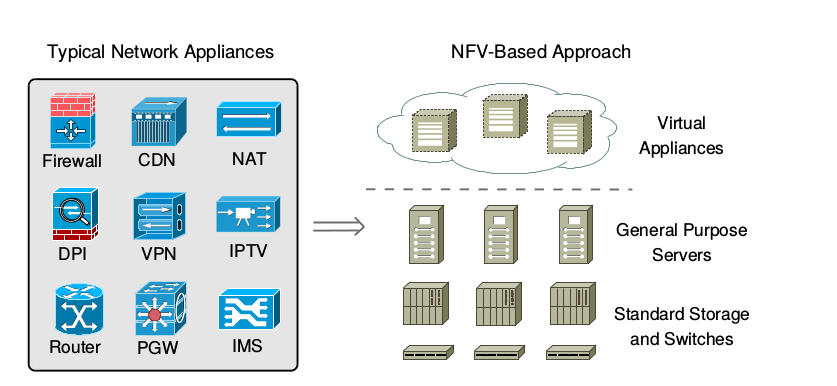
\includegraphics[scale=0.5]{images/vize_NFV}
\par\end{centering}
\caption{Koncept virtualizace síťových funkcí (NFV)\label{fig:vize_NFV}}
\end{figure}

Za zmínění stojí poznámka v \cite{NFVState}, kde je řečeno, že obecný koncept oddělení síťové funkce od hardwaru ještě nutně neznamená potřebu využití virtualizace. Protože budou síťové funkce dostupně jako software, tak mohou být nainstalovány a provozovány přímo na fyzickém stroji. Ovšem rozdíl je, že tento stroj již nebude speciální hardware, ale klasický server. Tento scénář může být do jisté míry použit při nasazovaní síťových funkcí v malém měřítku např. v uživatelských koncových bodech. Avšak pro plné využití všech výše zmíněných výhod, které jsou třeba ve velkých datových centrech, je třeba s použitím virtualizace počítat. To vše umocňuje fakt, že většina datových center v současnosti již využívá cloud computing. 

\section{Základní princip virtualizace}

Základním problém v tradičním modelu IT infrastuktury je, že servery podporují pouze jeden operační systém v čase. Na tomto systému obvykle běží pouze jedna aplikace. Přestože by na tomto systému popř. serveru mohlo běžet více aplikací, tak je lepší držet aplikace odděleně na různých systech z důvodu minimalizace potencionálních bodů selhání. Pokud například nastene s aplikací problém, tak častým řešením je restartování systému. Pokud by na systému bylo více aplikací, znamenalo by to jejich vyřazení z provozu po dobu restartu, který může trvat velice dlouho. \cite{VM_book}

Z výše zmíněných důvodů došlo k velkému rozvoji a nasazování virtualizace. Virtualizací obecně označujeme techniky, které umožňují k dostupným hardwarovým zdrojům přistupovat jiným způsobem, než jakým fyzicky existují. Je tomu díky softwaru, který tento hardware abstrahuje a vytvoří tím virtuální prostředí. Virtualizované prostředí se dá snadněji přizpůsobit potřebám uživatelů, případně skrýt pro uživatele nepodstatné detaily (jako např. rozmístění hardwarových prostředků). Tím je tedy umožněno na jednom fyzickém serveru provozovat více od sebe oddělených virtuálních strojů, které mají každý svůj vlastní operačních systému s aplikacemi. Software pro virtualizaci se nazývá hypervisor.\cite{VM_book}

Jak zmiňuje \cite{VM_architektura}, tak existují tyto dva základní typy hypervisorů:

\begin{itemize}
\item Typ 1 (Nativní) - Tento hypervisor běží přímo na fyzickém hardwaru. Tím umožňuje provozovat více operačních systému na jednom fyzickém stroji. Příkladem takového hypervisoru je VMware ESXi a XEN.
\item Typ 2 (Hostovaný) - Na rozdíl od předchozího případu tento typ hypervisoru běží v prostředí operačního systému. Příkladem je například KVM či Microsoft Hyper-V
\end{itemize}

\begin{figure}[h]
\begin{centering}
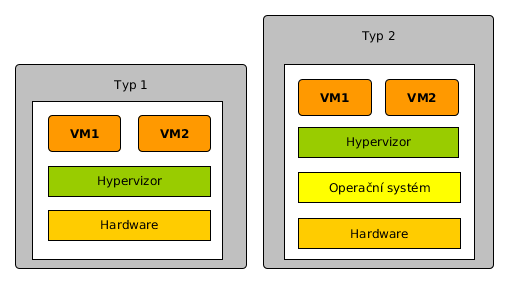
\includegraphics[scale=0.5]{images/virtualization}
\par\end{centering}
\caption{Schéma hypervisorů \label{fig:virtualization}}
\end{figure}

Obrázek \ref{fig:virtualization} zobrazuje schématický popis obou hypervisoru a jejich rozdíl. Problematika virtualizace je velice rozsáhlá a více informací o ní poskytují zdroje \cite{VM_book} a \cite{VM_architektura}.

\section{Cloud Computing}

Jak již bylo zmíněno, tak cloud computing, nebo někdy také označován pouze jako cloud, je oblast, ve které je velký potenciál pro využití virtuálních síťových funkcí. Z tohoto důvodu bude v této části jeho problematika přiblížena.

Cloud je technologie, kterou v poslední době začala provozovat většina větších organizací, jak ukazuje \cite{Cloud_adoption}. Cloud Computing má mnoho definic. Dle definice uvedené v \cite{Cloud_book} ho lze charakterizovat jako poskytování služeb, programů a výpočetních zdrojů servery dostupnými z internetu s tím, že uživatelé k nim mohou přistupovat vzdáleně.

Z technického hlediska tvoří cloud veškeré služby poskytované přes Internet a zároveň i infrastruktura, která tyto zdroje poskytuje. Tuto infrastrukturu tvoří velké množství fyzických serverů, které jsou vzájemně propojeny. Na těchto serverech běží hypervisor, který vytvoří virtuální infrastrukturu. Pro vytváření cloudových služeb zde musí ještě existovat cloudová platforma, která dokáže celou tuto virtuální infrastrukturu spravovat. \cite{Cloud_book}

Dle \cite{Cloud_book} existuje 5 základních atributů, kterými se cloud computing vyznačuje. Jsou to tyto:

\begin{itemize}
\item Služby dostupné na požádání
\item Všudypřítomný síťový přístup
\item Sdílení zdrojů
\item Vysokou elasticitu
\item Měření využitých zdrojů
\end{itemize}

\subsection{Distribuční modely}

Dle \cite{CloudSurvey} lze cloudové služby lze rozdělit do 3 základních kategorii. V \cite{NFV_use_cases} jsou k těmto kategorii přiřazeny příklady užití z oblasti virtualizace síťových funkcí. 

\begin{itemize}
\item Infrastracture as a Service (IaaS) - Nejzákladnější  model  poskytování  cloudových  služeb. IaaS cloudové platformy nabízejí například výpočetní výkon, virtuální disky, blokové a souborové úložiště či virtuální sítě.  Poskytovatelé  IaaS  cloudových  platforem  poskytují tyto zdroje na vyžádání ze svých datových center. Toto je možné díky skupiny hypervisorů v rámci cloudu, které mohou provozovat velké množství virtuálních strojů  a  mají  schopnost  škálovat  poskytované  služby v  závislosti  na  měnících  se požadavcích přicházejících od zákazníků. Tento model může tedy sloužit i pro poskytnutí všech potřebných zdrojů celé infrastruktury pro virtualizaci síťových prvků, neboli Network Function Virtualization Infrastrakture as a Service. Zde má uživatel pod nejvíce možností, jak navrhnout a spravovat virtuální síťové funkce, protože v zásadě dokáže nasazovat i vlastně navržené síťové funkce a nejen ty, které mu poskytuje provozovatel cloudu.
\item Platform as a Service (PaaS) - V  modelu  Platforma  jako  služba  (PaaS)  hostují  poskytovatelé cloudových  služeb určitou počítačovou  platformu, kterou následně poskytují koncovým uživatelům přes Internet. Tato platforma většinou bývá prostředí nějakého operačního systému, prostředí  pro  běh  určitého programovacího  jazyka,  databáze  a  webový  server.  Vývojáři  aplikací tím pádem  mohou provozovat a případně vyvíjet svá softwarová řešení bez výrazných nákladů a složitého nákupu a konfiguraci potřebného hardwaru a softwaru. Některé PaaS platformy nastavuje výpočetní  a  úložné  prostředky  aplikace  automaticky  tak,  aby  odpovídala  aktuálním požadavkům aplikace bez nutnosti zásahu zákazníka. NVF v tomto modelu může nabízet síťové služby, které se mohou skládat z více virtuálních síťových funkcí, neboli Virtual Network Platform as a Service. Zde je poskytnuta uživately velká kontrola nad konfigurací a ovládáním celé platformy.
\item Software as a Servicec (SaaS) - V modelu SaaS provozují poskytovatelé cloudových služeb aplikační software v cloudu a uživatelé  k  tomuto  softwaru  přistupují  pomocí  klientského  software  (např.  webové prohlížeče). Uživatelé  cloudu tedy  nespravují infrastrukturu  ani platformu, kde aplikace běží.  Není  proto  třeba zde nic instalovat  a  spouštět  aplikace  na  vlastních  počítačích uživatele, což velmi zjednodušuje údržbu. Cloudové aplikace se liší od ostatních aplikací v možnostech  škálování, kterého  může  být  dosaženo  díky  distribuci  úkolů  na  více virtuálních strojů, a tím reagovat na měnící se poptávku. Tento proces je pro uživatele služby transparentní, uživatel vidí pouze jeden přístupový bod pro danou aplikaci. Do této kategorie služeb může patřit poskytování virtuálních síťových funkcí, která je pouze ve formě softwarové aplikace, neboli VNFaaS. Takovéto aplikace poskytují síťovou funkci pro síťové správce a uživatele nejčastěji v privatním cloudu. 
\end{itemize}

\subsection{Modely nasazení}

Existuje několik základních modelů nasazení cloud computingu resp. cloudových platforem, které uvádí \cite{CloudSurvey}. V \cite{NFV_use_cases} lze k nim opět najít určité příklady z oblasti virtualizace síťových funkcí.

\begin{itemize}
\item Privátní cloud - Privátní cloud je  infrastruktura  provozována  výhradně  v  rámci  jedné  organizace. Může být spravován interně nebo prostřednictvím třetí strany a hostování může být opět interní nebo externí.  Aby  mohl  podnik  využít  privátní  cloud,  musí  nejprve  navrhnout a uzpůsobit k tomuto účelu svoji stávající infrastrukturu, která musí být virtualizována.  Vlastní  přechod  vyvolává  řadu  bezpečnostních  otázek,  které  je třeba řešit, aby se zabránilo vážným zranitelnostem celého řešení. Privátní cloud je přesně ten typ modelu, kde lze najít využití pro virtualizaci síťových funkcí.
\item Veřejný cloud - Veřejné cloudové jsou cloudové služby, jako jsou aplikace, výpočetní výkon, úložiště a další, které jsou k dispozici široké  veřejnosti.  Služby  jsou  poskytovány  zdarma  nebo  podle modelu  platby  za  množství  použitých  služeb.  Je  zvykem,  že  veřejní  poskytovatelé cloudových  služeb,  jako  je  Amazon  AWS,  Microsoft  nebo  Google,  vlastní  a  provozují hardwarovou infrastrukturu a nabízejí k ní přístup pouze přes Internet. V tomto modelu není očekáváno využívání NFV.
\item Hybridní cloud - Hybridní  cloud je  spojení  dvou  nebo  více  cloudů  (soukromých,  komunitních  nebo veřejných),  které  zůstávají  samostatné,  ale  jsou  těsně  propojeny.  Toto  složení  rozšiřuje možnosti  nasazení  cloudových  služeb  a  tím  umožňuje  IT  organizacím  využít  veřejné cloudové prostředky k uspokojení dočasných potřeb. Tato schopnost umožňuje hybridním cloudům škálovat přes více nezávislých cloudů. V tomto modelu může být využito NFV především na straně soukromého cloudu.
\item Komunitní cloud - V rámci komunitního cloudu sdílí infrastrukturu cloudu několik organizací, které mají společné zájmy (bezpečnost, dodržování předpisů, působnost, atd.). Komunitní cloud může být spravován interně nebo prostřednictvím třetí strany. Náklady jsou rozloženy mezi méně uživatelů než na veřejném cloudu. V tomto modelu může být využito NVF, pokud se provozovatelé takovéhoto cloudu domluví. 
\end{itemize}


\section{Souvislost NFV a SDN} \label{sub:SDN}

Softwarově definované sítě (SDN) je další z nových technologii, která se snaží vylepšit a automatizovat správu stávajících počítačových sítí. Dle \cite{SDN_clanek} jde o koncept, ve které je oddělena řídící logika (control plane) z jednotlivých routerů a switchů, které přeposílají traffic (data plane). Tím, že dojde k oddělení datové a řídící vrstvy, se routery a switche stanou pouze přeposílající data a veškerá řídí logika může být implementována v jednom logicky centrálním místě (SDN Controller). Z tohoto centrálního místa lze do jednotlivých routerů a switchů předávat instrukce pomocí aplikačních programovacích rozhraní (API). Samotný SDN Controller také obsahuje API, které mohou využívat aplikace a tím řídit, resp. programovat celou počítačovou síť.

\begin{figure}[h]
\begin{centering}
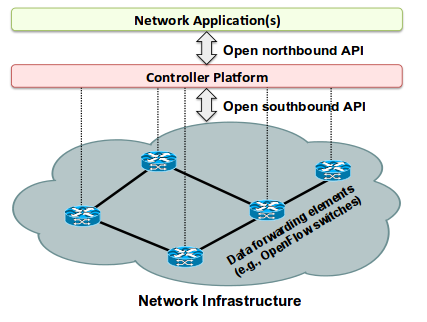
\includegraphics[scale=0.60]{images/SDN}
\par\end{centering}
\caption{Schéma SDN, převzato z \cite{SDN_clanek}\label{fig:SDN}}
\end{figure}

Obrázek č. \ref{fig:SDN} úkazuje jednoduché schéma softwarově definovaných sítí. Celou architekturu lze tedy rozdělit do 3 logických vrstev, které spolu komunikují pomocí API. 

\begin{itemize}
\item Aplikační vrstva - Na této úrovni se nachází samotné síťové aplikace jako jsou například DHCP, ACL, NAT, DNS a další. Jejich vytváření by
mělo být poskytováno prostřednictvím nižší vrstvy, nazývané northbound API.
\item Northbound APIs - Toto API využívají aplikace pro komunikaci s SDN controllerem. 
\item Control vrstva - V této vrstvě je centralizována veškerá logika, které dříve byla v síťových prvcích.
\item Southbound APIs - Jedná se o skupinu API protokolů, které pracují mezi vrstvou infrastruktury a control vrstvou. Jejím hlavním úkolem je komunikace, která povoluje SDN controleru instalovat na samotné síťové prvky rozhodnutí definované v aplikační vrstvě.
\item Vrstva infrastruktura - Nejnižší vrstvou je samotný hardware pro předávání datagramů na fyzické úrovni. Pro funkčnost celé architektury je nutné, aby zde byla nasazena zařízení, která umí přijímat pokyny od control plane skrze southbound API.

\end{itemize}


Přestože Softwarově definované sítě a virtualizace síťových funkcí jsou dvě různé technologie a koncepty, tak se navzájem se doplňují. Fakt, že SDN umožňuje programaticky ovládat počítačovou síť, lze využít pro poskytnutí programovatelné konektivity mezi jednotlivými virtuálními síťovými funkcemi. Naopak SDN může využít NFV tím, že implementuje potřebné síťové funkce jako software. Může tak virtualizovat SDN Controller, který tak může běžet na co nejvhodnějším místě v datovém centru. Je vidět, že tyto dvě technologie se dobře doplňují, proto jsou často součástí jednoho řešení. \cite{SDN_book}


\subsection{Service Chaining}

Jednou z výhod NFV je možnost využít Service Chaining. Service chaining je ve skutečnosti součást SDN. Jde o princip jakým lze dynamicky pospojovat jednotlivé VNF a ovladat tak toky v síti. \cite{SDN_book}

Service chaining není ve skutečnosti nic nového. V klasických počítačových sítích je používán také, ale pomocí fyzických síťových prvků. Jedná se zjednodušeně o způsob zapojení mezi jednotlivými síťovými prvky (či VNF) a způsob, jakým na sebe navazují. Příklad takového zapojení je vidět na obrázku č. \ref{fig:service_chaining}. Zde se provozovatel sítě rozhodl, že odchozí data z klientských stanic musí jít přes firewall, IDS a nakonec přes NAT do Internetu. Příchozí data mají logicky obrácené pořadí. Toto zapojení funguje dobře pro síť, kde není třeba rozlišovat cestu jakou proudí data jednotlivých uživatelských stanic. Ale není to optimální řešení pro sítě s více uživateli, kde každý požaduje jinou síťovou funkci. Potřeba jednotlivých síťových služeb se samozřejmě může v čase měnit. Příklad takové sítě lze nalézt ve většině datových center. 

\begin{figure}[h]
\begin{centering}
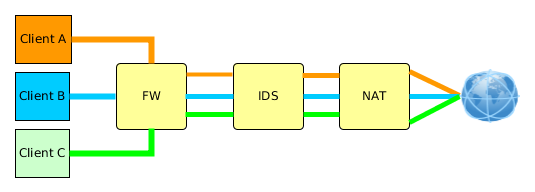
\includegraphics[scale=0.55]{images/service_chaining}
\par\end{centering}
\caption{Ukázka klasického service chainigu pomocí fyzických síťových prvků\label{fig:service_chaining}}
\end{figure}

Zde tedy přichází na řadu VNF spolu s SDN. Protože jednotlivé VNF existují jako virtuální stroje, tak mohou být dynamicky nasazovány dle aktuálním požadavků jednotlivých klientů a pomocí SDN mohou být tyto VM dynamicky pospojovány. Obrázek č. \ref{fig:service_chaining_new} ukazuje schéma zapojení, kde každý klient může mít jinou požadovanou cestu do internetu. Je možná i varianta, kde každý klient má své vlastní VNF s jinou konfigurací.

\begin{figure}[h]
\begin{centering}
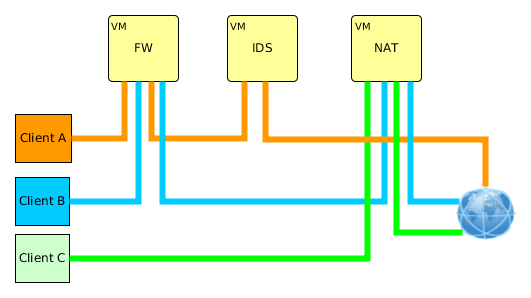
\includegraphics[scale=0.55]{images/service_chaining_new}
\par\end{centering}
\caption{Ukázka VNF service chainigu\label{fig:service_chaining_new}}
\end{figure}

\section{Architektura NFV a VNF} \label{sub:architektura}

V předchozí sekci byla popsána myšlenka a motivace související s virtualizací síťových funkcí. Protože cílem této práce je navržení jednoduchého NFV frameworku, tak je nejprve nutné se seznámit s jeho obecnou architekturou. V této práci se bude vycházet z referenční architektury NVF \cite{NFV_architektura}, která byla navržena organizací ETSI. Jedná se pouze o funkční návrh bez náznaků konkrétní implementace. Od této skupiny existují i podrobnější návrhy jednotlivých částí celého NFV frameworku, které v této práci budou také popsány v příslušných kapitolách.

\begin{figure}[h]
\begin{centering}
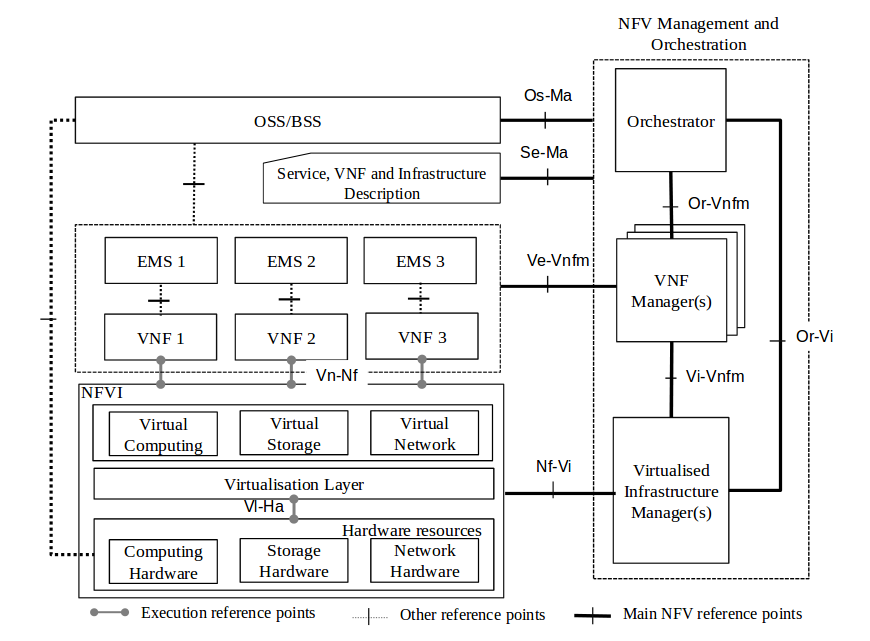
\includegraphics[scale=0.5]{images/NFV_architektura}
\par\end{centering}
\caption{NFV architektura, převzato z \cite{NFV_architektura}\label{fig:NFV_architektura}}
\end{figure}

Jak je vidět na obrázku č. \ref{fig:NFV_architektura}, tak celá architektura se dá rozdělit na tyto 3 hlavní části:

\begin{itemize}
\item Infrastruktura virtualizace síťových funkcí (NFVI) - Jsou všechny softwarové a hardwarové zdroje potřebné k vytvoření prostředí, ve které mohou být jednotlivé VNF být nasazeny. Tato infrastruktura může být velice rozsáhlá, proto je její součástí i síť poskytující konektivitu mezi vzdálenými lokacemi infrastruktury.\cite{NFV_terminology}
\item Virtualizované síťové funkce (VNFs) - Jsou softwarové implementace síťových funkcí, jako je např. NAT a routing. které mohou být nasazeny na NFV infrastruktuře.
\item Management a orchestrace NFV (NFV-MANO) - zde se jedná o řízení softwarových a hardwarových zdrojů v celé infrastruktuře NFV a životního cyklu jednotlivých virtuálních síťových funkcí. Tato část se tedy zaměřuje na řízení a správu všech úloh související v virtualizací v NFV frameworku. \cite{NFV_terminology}
\end{itemize}

Tyto funkční bloky se ještě dále dělí, proto dále v této práci budou tyto jednotlivé části popsány podrobněji a současně k nim budou uvedeny různé možnosti řešení.

\subsection{Infrastruktura NFV}

Ve zdroji \cite{NFV_infrastructure}, který detailně popisuje infrastrukturu pro virtualizaci síťových funkcí (NFVI), je uvedeno, že je v ní sdružení všech základních zdrojů potřebných pro běh virtuálních síťových funkcí (VNF). Z tohoto důvodu sem patří veškerý hardware. Do NFVI také patří některé softwarové komponenty, které jsou společné mnoho VNF a poskytují funkcionalitu potřebnou pro podporu nasazení, propojení či managementu VNF. Celou infrastrukturu může tvořit jeden či více strojů, které mají tyto potřebné funkce. Tyto stroje také mohou být umístěny v různých spolu spojených lokacích. 

Pro zjednodušení lze celou NFV infrastrukturu rozdělit do 3 následujících domén:

\begin{itemize}
\item Compute Domain - Do této domény patří veškeré hardwarové zdroje jako jsou servery, úložiště a komponenty, které tyto zdroje obsahují, např. procesory, pevné disky, síťové karty, atd. Zároveň je zde řešen návrh fyzické topologie. \cite{NFV_compute}
\item Hypervisor Domain - Toto je doména, které představuje softwarové prostředí abstrahující hardware v compute doméně a poskytuje je jako virtuální zdroje. Tyto zdroje následně mohou využívat virtuální síťové funkce. \cite{NFV_hypervisor}
\item Infrastructure Network Domain - V této doméně je řešeno veškeré propojení výše zmíněných domén. Tedy fyzické i virtuální infrastruktury.\cite{NFV_network}
\end{itemize}

Funkci obsaženou v jednotlivých doménách znázorňuje obrázek č. \ref{fig:infrastruktura}. Více informací na tuto problematiku lze nalézt v \cite{NFV_infrastructure} a ve zdrojích uvedených u každé domény. 

\begin{figure}[h]
\begin{centering}
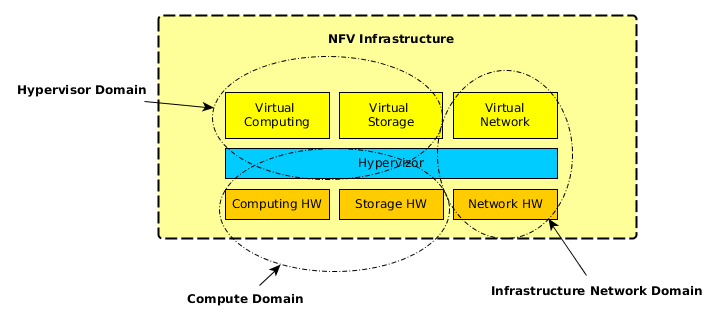
\includegraphics[scale=0.65]{images/infrastruktura}
\par\end{centering}
\caption{Schéma NFV infrastruktury\label{fig:infrastruktura}}
\end{figure}

Dá se říci, že referenční návrh infrastruktury pro NVF je podobný jako pro návrh infrastruktury pro cloud computing platformu. Měl by se tedy skládat z generických a komerčně vysoce dostupných serverů, které by měli být zapojeny do switche a tím by měla být zajištěna konektivita. Na tyto servery je následně nasazen jeden z dostupných hypervisorů. Výběr správného hypervisoru, které jsou v současné době dostupné na trhu, je hlavní podmínka správného a funkčního návrhu této části NFV frameworku. Přehled hypervisorů je uveden v kapitole \ref{sub:Hypervisor}. V produkčním prostředí by součástí řešení bylo samozřejmě řešení síťového návrhu. Tato práce však má sloužit pouze jako ukázka a z tohoto důvodu zde nebude síťový návrh zmíněn.

\subsection{Virtuální síťová funkce}

Virtuální síťová funkce (VNF) je dle \cite{NFV_VNF} určitá síťová funkce, která běží na NVF infrastruktuře a je zároveň NVF frameworkem řízena a spravována. Zároveň musí mít dobře definované rozhraní k ostatním síťovým funkcím, k VNF Managerovi a měla by obsahovat management rozhraní či port. Jedna VNF může být být obsažena v jednom virtuálním stroji nebo může být roztažena přes více virtuálních strojů. 

Na obrázku č. \ref{fig:VNF} je vidět jednoduché schéma virtuální síťové funkce dle referenčního návrhu \cite{NFV_VNF}. Celý životní cyklus VNF, což je vytvoření, spuštění, zastavení, smazání a škálování, řídí VNF Manager, který je součástí NVF managementu a orchestrace. Současně je možné dynamicky změnit aktuální konfiguraci pomocí Entity manageru (EM) přes management interface. EM může spravovat více VNF nebo právě jednu. Vnitřní struktura celé instance může být tvořena více komponentami (VNFC), které spolu mohou být navzájem provázány. Toto provázání však nemusí být viditelné zvenčí.

\begin{figure}[h]
\begin{centering}
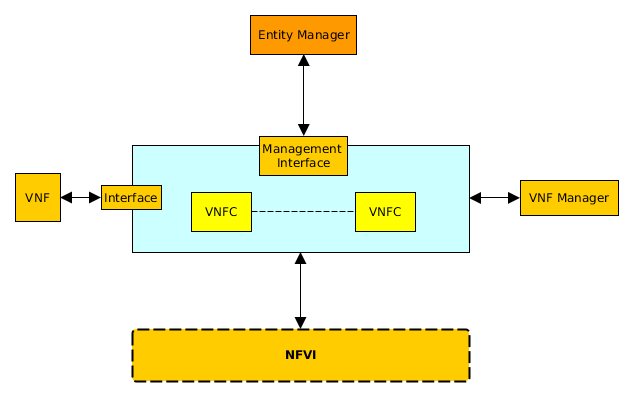
\includegraphics[scale=0.67]{images/VNF}
\par\end{centering}
\caption{Schéma virtuální síťové funkce\label{fig:VNF}}
\end{figure}

Pohledem na současný trh zjistíme, že VNF je prakticky poskytována ve 3 základních podobách.

\begin{itemize}
\item Softwarová aplikace - V tomto případě je poskytována VNF jako aplikace, která může být nainstalována na běžný operační systém jako je například GNU/Linux.
\item Ucelený operační systém - Zde je poskytován přímo celý operační systém, který může být nainstalován do virtuálního stroje nebo i na fyzický server.
\item Kompletní VM - Poskytovatel VNF může dát k dispozici rovnou přetvořený obraz virtuálního stroje (image), který může obsahovat operační systém se síťovými funkcemi. Tento systém však nemusí být klasicky dostupný operační systém jako je GNU/Linux či FreeBSD, ale může se jednat o speciálně vytvořený systém od výrobce. Tento způsob budou využívat poskytovatelé, kteří mají proprietární řešení pro síťová řešení jako je například Cisco či Juniper.
\end{itemize}


\subsection{Management a orchestrace NFV}

Management a orchestrace virtualizace síťových funkcí (NFV MANO) je nejdůležitější část celého NFV frameworku. Je tomu tak, protože MANO zajišťuje správné fungování NFV infrastruktury i jednotlivých virtuálních síťových funkcí. MANO také poskytuje funkce nutné pro provisioning VNF a související operace, jako je jejich konfigurace jednotlivých VNF a infrastruktury, na které běží. Zároveň spravuje a řídí životní cyklus fyzických a virtuálních zdrojů, které slouží pro podporu VNF. 

\begin{figure}[h]
\begin{centering}
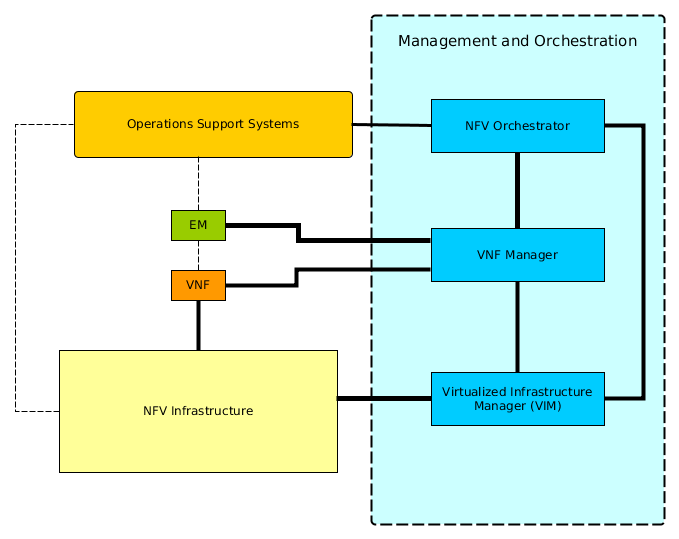
\includegraphics[scale=0.65]{images/MANO}
\par\end{centering}
\caption{Schéma NFV MANO\label{fig:MANO}}
\end{figure}

Jak vyplývá z obrázku č. \ref{fig:MANO}, tak referenční návrh MANO dle \cite{NFV_MANO} se skládá ze hlavních 3 částí, které se zabývají správnou jednotlivých vrstev NFV frameworku.

\begin{itemize}

\item Virtualized infrastructure manager (VIM) - Řídí a spravuje fyzické a virtuální zdroje v jedné doméně infrastuktury. Celková infrastruktura se může skládat z více domén a každá musí mít svůj VIM. Jeho typickými úlohami jsou vytvýření, udržování a uvolňování VM na dostupných zdrojích v doméně. Zároveň musí mít přehled o všech těchto a stavu hardwarových zdrojů.

\item VNF manager - Dohlíží na lifecycle management jednotlivých VNF instancí. To znamená, že výtváří, udržuke a ukončuje VNF instance, které běží na jednotlivých VM (ty však spravuje VIM). Opět může existovat více VNF managerů, kteří mohou spravovat jednu či více VNF.

\item NFV orchestator - Zjednodušeně slouží jako řízení a správu všech VIM a všech VNF managerů. Pomocí komunikace s VIM dokáže spravovat dostupné zdroje a pomocí komunikace s VNF managery dokáže řídit síťové služby. Jeho další funkcí je i přehled všech dostupných VNF, neboli katalog VNF, a registrace nových VNF do tohoto katalogu. Ten je pak dostupný uživatelům.
\end{itemize}

Celý systém je navržen tak, že by měl pracovat společně se stávajícími aplikacemi a systémy, které potencionální uživatelé používají pro provoz své infrastruktury a podnikových procesů (Operation support system).

V oblasti NFV MANO probíhá v součastnosti rozsáhlí vývoj a existuje několik projektů, které se tím zabývají. V článek \cite{NFV_orchestration} je nabídnut zajímavý přehled.


\section{Možné technologie pro řešení}

V předchozí části byla popsána referenční architektura, kterou navrhla ETSI. V té jsou specifikovány funkční požadavky a nastíněny potřebná rozhraní. Přesto lze tento návrh považovat za poněkud omezený v rozsahu. Není v něm například definována řízení a správa starších zařízení, což může velice zkomplikovat provoz síťové infrastruktury, která se skládá z VNF i těchto starších zařízení. Kromě toho standardy a referenční implementace VNF, infrastruktury, a MANO prozatím nejsou k dispozici.

Z tohoto důvodu následuje návrh možnosti pro každou z oblastí architektury, které v současnosti mohou sloužit jako její řešení.


\subsection{Hypervisory} \label{sub:Hypervisor}

hypervisor je základná součástí cloudové platformy a frameworku pro virtualizaci síťových funkcí. Na trhu již existuje celá řada různých hypervisorů. Zde je uveden stručný přehled těch nejpoužívanějších.

\begin{itemize}
\item XEN - Je to hypervisor prvního typu, který pracuje na nejnižší vrstvě. Tato vrstva podporuje jeden nebo více hostovaných operačních systémů. První hostovaný systém se nazývá doménou 0 a slouží k přímému přístupu k hardwaru a jeho management. Do tohoto systému následně je možné přidávat další uživatelské domény, které mohou být linuxové systémy či Microsoft Windows.
\item KVM - Jedná se o virtualizaci založenou na linuxovém jádru. Každá virtuální instance má svůj vlastní virtualizovaný hardware včetně síťové karty, disku a grafické karty. Tento typ hypervisoru vyžaduje pro správnou funkci procesor s rozšířením pro virtualizaci hardwaru.
\item Microsoft Hyper-V - Zde se jedná o hypervisor od společnosti Microsoft, který lze nalézt v Windows Serverech od verze 2008. Hyper-V je hypervisorově stavěný serverový systém. To znamená, že má svůj hlavní operační systém a pomocí virtualizace se skrze něj mohuo spustit další operační systémy. 
\item WMware ESXi - Varianta  ESXi  je  odlehčená  verze ESX  klienta,  která  dovoluje  běžet  hostitelský systém na výměnném zařízení. Jde o tenký klient s vlastním linuxovém jádrem, který běží přímo nad hardwarovou vrstvou. Kernel ESXi funguje jako hostitelský operační systém pro vrstvení dalších služeb. Kernel na sebe váže modul vmkernel s dalšími obslužnými funkcemi, který tvoří základní stavební kámen celého řešení. Výhodou tohoto řešení  je možnost alokace co  největšího  množství  hardwarových prostředků  pro hostované systémy.  Tenký  klient  totiž  zbytečně nevyužívá  systémové prostředky  hostujícího  serveru.

\end{itemize}

\subsection{VNF}

Pokud se podíváme na trh s VNF u některých vendorů, tak zjistíme, že mnozí poskytují virtuální instance, které se dají použít pro účely VNF v této práci. Tato práce je zaměřena především na funkce firewallu a proto zde jsou uvedeny příklady pouze pro ně. Uvedeny jsou hlavně produkty největších a nejpoužívanějších poskytovatelů síťových prvků a také open-source firewall.

\begin{itemize}
\item Juniper vSRX - Jde o firewall od společnosti Juniper, který je obdobou jejich fyzického zařízení Juniper SRX. Jde virtuální instanci poskytující funkce pro firewall, routing a pokročilé bezpečností funkce pro poskytovale telekomunikačních služeb a větší společnosti. Toto VM je určené pro privátní, public i hybrid cloud. 
\item Fortigate-VM - Fortigate Virtual Appliances je řešení pro cloudové prostředí od společnosti Fortinet. Nabízí stejně funkce pro firewall jako jsou obsaženy ve Fortigate fyzických zařízeních.
\item Cisco ASAv - Společnost Cisco nabízí Adaptive Security Virtual Appliance (ASAv), která obsahuje stejný software jako fyzické ASA zařízení a vetšinu funkcí pro firewall, routing a VPN. 
\item PFSense - PFSense je open-source projekt, který má za cíl poskytnout firewall postavený na operačním systému FreeBSD, který může běžet na klasické architektuře jednodeskových počítaču. Toto řešení poskytuje všechny důležité vlastnosti komerčních firewallů, má jednoduché ovládání a je to otevřené řešení.
\end{itemize} 

\subsection{Cloud platforma}

Pro účely vytvoření infrastruktury, a vůbec možnost využití NFV v datovém centru, je nutná cloudová platforma. Existují několik řešení, které lze pro tyto účely použít. Dvě z nejčastějších jsou OpenStack a VMware vCloud.


\subsubsection{OpenStack}

OpenStack je open-source platformou umožňující postavit IaaS cloud, který může být nainstalován i na běžném hardwaru. Toto řešení má za cíl vytvořit dostupnou cloudovou platformu, která bude splňovat všechny potřeby privátních a veřejných cloudů nezávisle na velikosti řešení.

Celá stavba systému OpenStack se skládá z několika na sobě nezávislých projektů, které řeší různé oblasti cloudové platformy. Tyto projekty mezi sebou komunikují pomocí otevřených API a mohou být spravovány pomocí dashboardu. Celé administrace OpenStacku může být prováděna přes webově rozhraní, příkazovou řádku či přímo pomocí příkazů zaslaných do API. Celé toto řešení se vyznačuje jednoduchostí implementace, škálovatelností a rychlým vývojem nových vylepšení. Toto

\subsubsection{VMware vCloud}

Společnost Vmware poskytuje pro privátní cloudové systémy své řešení, které označuje jako VMware vCloud. 

\subsection{SDN}

Součástí řešení pro datové centrum je dnes i SDN. I zde existuje několik možností. Dvě z nejpoužívanější řešení jsou:

\begin{itemize}
\item OpenContrail
\item VMware NSX
\end{itemize} 



\chapter{Popis použitých technologií a testovacího prostředí}

\section{OpenStack}\label{sub:interaction}

\subsection{}

\subsection{Heat Templates}

\begin{figure}[h]
\begin{centering}
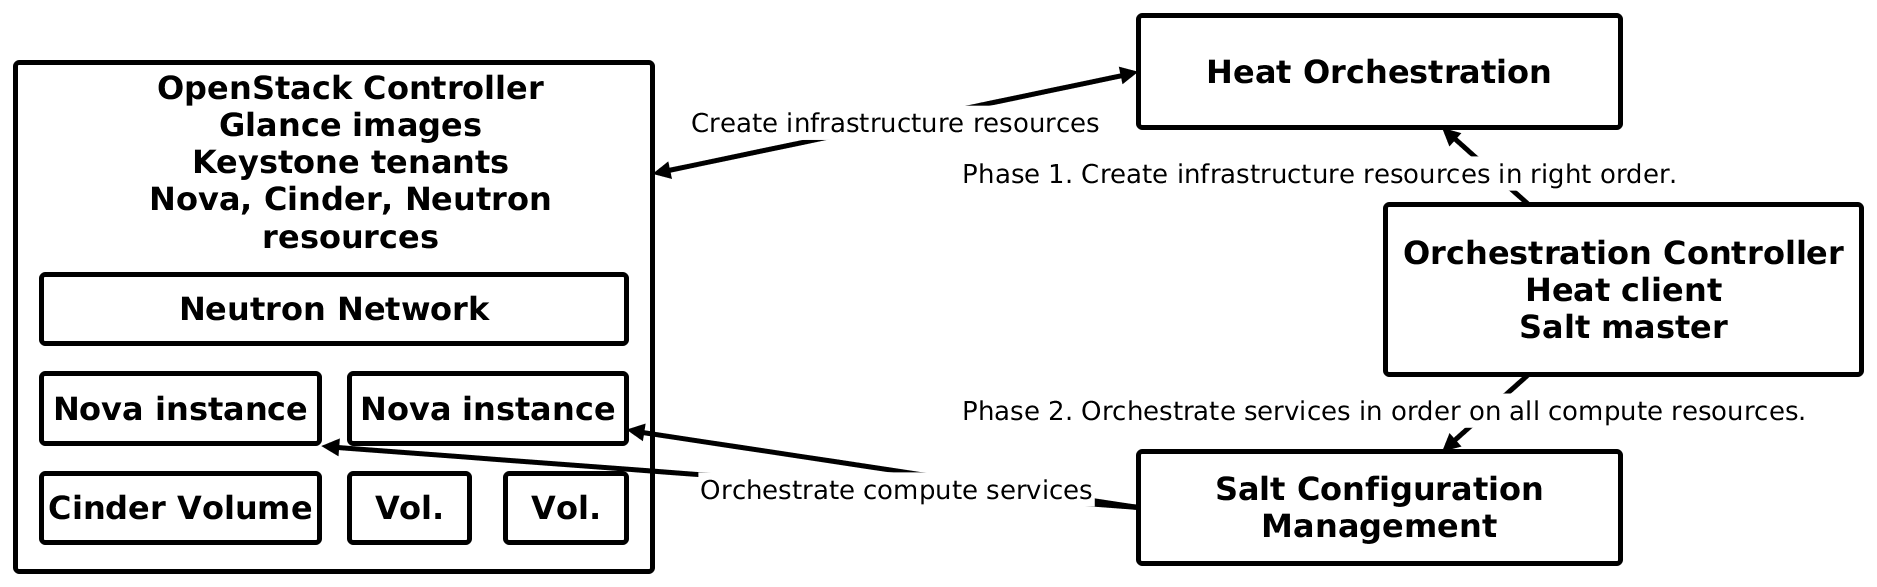
\includegraphics[scale=0.21]{images/heat}
\par\end{centering}
\caption{Popis heat orchestrace\label{fig:heat}}
\end{figure}

\section{OpenContrail}\label{sub:interaction}

\subsection{Service Chaining}

\section{Přehled testovací topologie}\label{sub:interaction}








\chapter{Virtuální síťové funkce (VNFs)}

V předešlé kapitole byla vysvětlena základní problematika, která souvisí s virtualizací síťových funkcí, cloud computingem a softwarově definovanými sítěmi. Zároveň byla popsána referenční architektura frameworku pro virtualizaci síťových funkcí. Tato kapitola bude již věnována konkrétnímu příkladu využití virtuálních síťových funkcí v cloudovém prostředí. Nejprve zde popsána navržená architektura pro privátní cloudovou platformu využívající virtualizaci síťových funkcí, kterou mohou využívat všichni její uživatelé. Pro tuto cloudovou platformu a pro její uživatele byli navrženy dva příklady virtuálních síťových funkcí. U obou příkladů jsou uvedeny scénáře a způsob jakým jsou navrženy.

\section{Požadavky na životní cyclu VNF}

//automatic creating of VNF + with all infrastructure

//automatic konfiguration + 

//automatic rekonfiguration

\section{Použité technologie}

\subsection{OpenStack}

//Todo Proč jsem si vybral OpenStack??

//Citace OpenStack a VNF.

OpenStack je open-source platformou umožňující postavit IaaS cloud, který může být nainstalován i na běžném hardwaru. Toto řešení má za cíl vytvořit dostupnou cloudovou platformu, která bude splňovat všechny potřeby privátních a veřejných cloudů nezávisle na velikosti řešení. \cite{OpenStack}

Celá stavba systému OpenStack se skládá z několika na sobě nezávislých projektů (modulů), které řeší různé oblasti cloudové platformy. Tyto projekty mezi sebou komunikují pomocí otevřených API a mohou být spravovány pomocí dashboardu. Celé administrace OpenStacku může být prováděna přes webově rozhraní, příkazovou řádku či přímo pomocí příkazů zaslaných do API. Celé toto řešení se vyznačuje jednoduchostí implementace, škálovatelností a rychlým vývojem nových vylepšení. Hlavními moduly OpenStacku jsou \cite{OpenStack} \cite{OpenStack2}:

\begin{itemize}
\item Keystone - identifikační služba používaná OpenStackem pro autorizaci a autentizaci. Ověřování probíhá pomocí tokenů. Uživatel přihlášením odesílá žádost na Keystone, který tento modul zpracuje, zjistí pověření a vytvoří token. Vytvořený token je poté odesílán s žádostí do ostatních služeb. Zde dojde ke komparaci tokenu se současnou přístupovou politikou a dojde ke zjištění, zdali má uživatel dostatečná oprávnění pro provedení požadovaného úkonu.
\item Glance - služba umožňující práci s virtuálními diskovými obrazy (imagy). Tyto obrazy mohou být uloženy na mnoha různých místech od lokálních systémových disků až po distribuované souborové systémy, jako je OpenStack Storage.
\item Nova - tento modul poskytuje výpočetní služby. Umožňuje tedy běh několika instancí virtuálních strojů na několika hostitelských strojích, nan kterých je nainstalována služba OpenStack compute. OpenStack podporuje hypervizory KVM, QEMU, VMware ESX, Hyper-V, Xen. 
\item Neutron - je služba pro správu všech síťových aspektů OpenStacku. Jedná se tedy o SDN komponentu. Neutron podporuje možnost rozšíření o tzv. pluginy, které umožňují využívat řešení třetích stran pro síťování.
\item Cinder - poskytuje infrastrukturu pro mapování volumů v OpenStacku.
\item Ceilometer - služba, která sbírá měřená data a monitoruje tak využívané zdroje.
\item Heat - umožňuje automatizovanou orchestraci virtuálních strojů na základě vytvořených templatů.
\item Horizon - představuje dashboard, který umožňuje cloudovým administrátorům a uživatelům spravovat různé zdroje a služby OpenStacku. Dashboard umožňuje interakci s OpenStackovým kontrolerem prostředníctvím API. 
\end{itemize}

\subsubsection{Heat}

\subsection{OpenContrail} 

OpenContrail je systém, který může být použit v mnoha síťových scénářích jako například v cloud networkingu nebo v sítích poskytovatele síťových služeb. V privátním cloudu, ve Virtual Private Cloud (VPC) a v IaaS se vyskytuje prostředí s velkým množstvím tenantů, kde několik tenantů sdílí stejné fyzické zdroje (server, uložiště, fyzickou síť). Každý tenant má přiřazeny vlastní logické zdroje (virtuální stroje, virtuální uložiště, virtuální sítě). Tyto logické zdroje různých tenantů musí být od sebe odděleny. Virtuální sítě v datacentrech mohou být také spojeny s fyzickou IP VPN nebo L2 VPN. \cite{OpenContrail}

OpenContrail je složen ze dvou hlavních komponent. První z nich je Controller, který je logicky centralizovaný, ale fyzicky distribuovaný. To znamená, že je složen z několika typů rolí a každý z nich má několik instancí z důvodu vysoké dostupnosti a horizontální škálovatelnosti. Tyto role mohou být fyzické servery nebo virtuální stroje. Tyto role jsou \cite{OpenContrail2}: 

\begin{itemize}
\item Configuration role - poskytuje north-bound REST API. Toto API může být použito pro konfiguraci systému nebo pro extrahování operačního stavu systému.
\item Control role - implementuje logicky centralizovanou část control planu.
\item Analytics role - je zodpovědný za sběr, porovnání a prezentaci analytických informací.
\end{itemize}

Další komponentou je vRouter, který má na starost přenos dat. VRouter běží na virtualizovaném serveru, na kterém běží hypervizor. Rozšiřuje fyzickou síť v datovém centru o virtuální overlay síť hostovanou ve virtualizovaných serverech. VRouter narozdíl od vSwitchů poskytuje směrování a služby vyšších vrstev. Data plane, tedy vRoutery mezi sebou, může používat různé technologie overlay jako MPLS over GRE, MPLS over UDP a VXLAN. Control plane protocol mezi Controllerem a fyzickým gateway routerem (nebo switchem) je BGP. Protokol používaný mezi Controllerem a vRoutery se nazývá XMPP. Obrázek č. \ref{fig:contrail} ukazuje schéma OpenContrailu.

\begin{figure}[h]
\begin{centering}
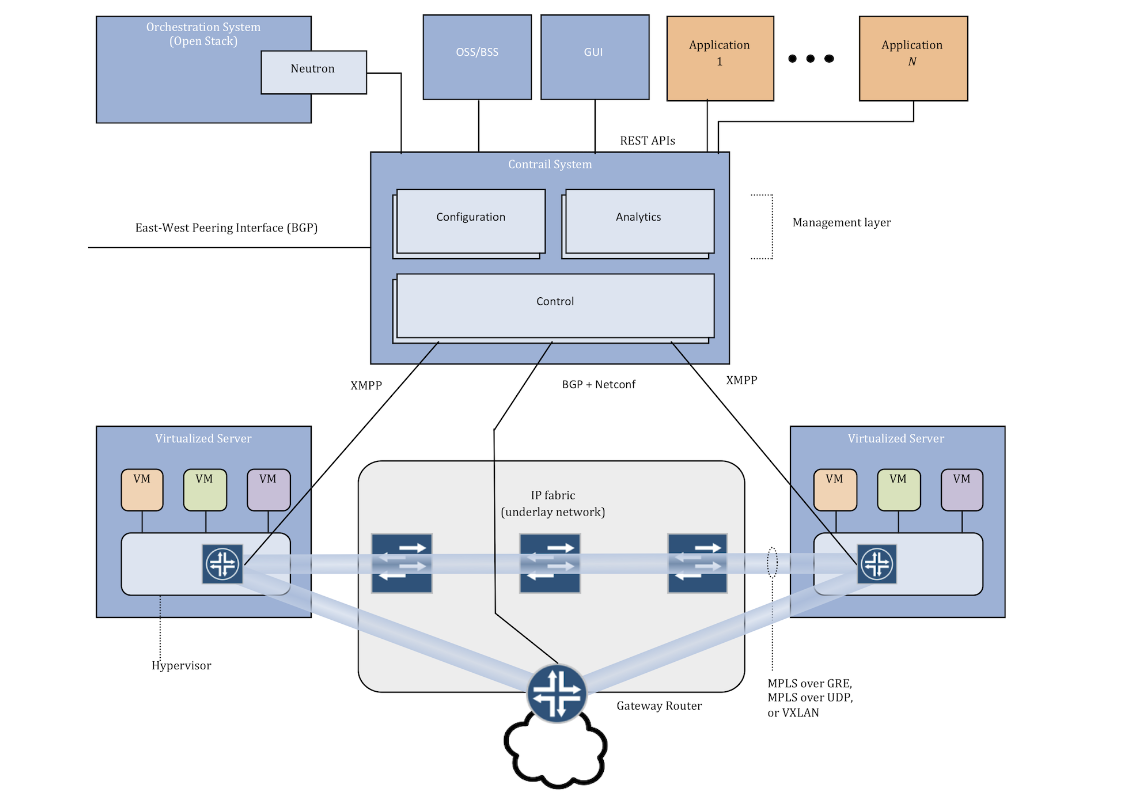
\includegraphics[scale=0.35]{images/contrail}
\par\end{centering}
\caption{Schéma OpenContrail, převzato z \cite{OpenContrail}\label{fig:contrail}}
\end{figure}

//Servisní instance v Opencontrailu

\subsection{SaltStack}

\subsection{Použitý software pro VNF}

//TODO co jsem si vybral za VNFka

Pokud se podíváme na trh s VNF u některých vendorů, tak zjistíme, že mnozí poskytují virtuální instance, které se dají použít pro účely VNF v této práci. Tato práce je zaměřena především na funkce firewallu a proto zde jsou uvedeny příklady pouze pro ně. Uvedeny jsou hlavně produkty největších a nejpoužívanějších poskytovatelů síťových prvků a také open-source firewall.

\begin{itemize}
\item Juniper vSRX - Jde o firewall od společnosti Juniper, který je obdobou jejich fyzického zařízení Juniper SRX. Jde virtuální instanci poskytující funkce pro firewall, routing a pokročilé bezpečností funkce pro poskytovale telekomunikačních služeb a větší společnosti. Toto VM je určené pro privátní, public i hybrid cloud. 
\item Fortigate-VM - Fortigate Virtual Appliances je řešení pro cloudové prostředí od společnosti Fortinet. Nabízí stejně funkce pro firewall jako jsou obsaženy ve Fortigate fyzických zařízeních.
\item Cisco ASAv - Společnost Cisco nabízí Adaptive Security Virtual Appliance (ASAv), která obsahuje stejný software jako fyzické ASA zařízení a vetšinu funkcí pro firewall, routing a VPN. 
\item PFSense - PFSense je open-source projekt, který má za cíl poskytnout firewall postavený na operačním systému FreeBSD, který může běžet na klasické architektuře jednodeskových počítaču. Toto řešení poskytuje všechny důležité vlastnosti komerčních firewallů, má jednoduché ovládání a je to otevřené řešení.
\end{itemize} 

Navrhnutá řešení v této práci předvádějí virtuální víťové funkce pro firewall a load balancing. Jsou zde ukázány celkem 3 scénáře případu užíti. Dva jsou zaměřeny na FwaaS (Firewall as a Service) a jeden na LbaaS (Load balancer as a Service). Všechna řešení jsou vytvořena pomocí Heat templatů, které se spouští v prostředí OpenStack.

Aby mohla být nějaká VNF vůbec vytvořena, tak musel být nejprve zvolen software či operační systěm, který má požadovanou funkci implementovánu. Pro tyto účely byly použity následující řešení:

\begin{itemize}
\item PFSense – open-souce firewall založený na operačním systému FreeBSD.
\item FortiGate-VM – je plnohodnotně vybavený Fortigate firewall zabalený jako virtualní instance.
\item Neutron Agent-HAproxy – je velmi rychlé a spolehlivé řešení nabízející vysokou dostupnost, load balancing a proxy pro aplikace založené na TCP a HTTP
\end{itemize}

Následující diagram znázorňuje logickou architekturu navrženého řešení dle referenční architektury zmíněné v kapitole 2.4. OpenStack spolu s OpenContrailem poskytují NFV infrastrukturu jednotlivé VNF jsou řízeny pomocí Heat.

\section{Architektura použitého frameworku}

Architektura navrženého řešení byla implementována pomocí cloudové platformy OpenStack a SDN řešení OpenContrail. Obrázku č. \ref{fig:VNF_overview} znázorňuje tyto technologie v souvislosti s referenční architekturou popsanou v kapitole \ref{sub:architektura}. Je nutné říci, že obě technologie nezapadají přímo do jedné z částí referenční architektury. Naopak v některých případech se překrývají nebo se v ní doplňují.

\begin{figure}[h]
\begin{centering}
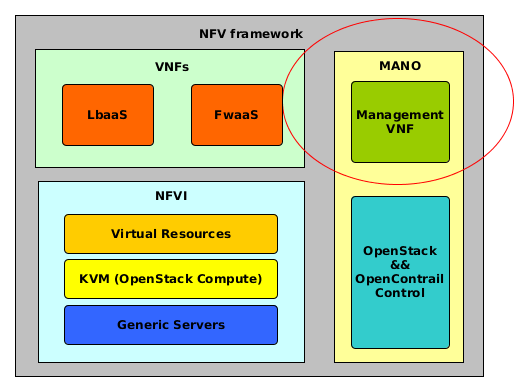
\includegraphics[scale=0.51]{images/VNF_overview}
\par\end{centering}
\caption{Architektura NFV řešení\label{fig:VNF_overview}}
\end{figure}

OpenStack byl zvolen, protože se jedná o největší open-source cloudovou platformu na světě. OpenStack tvoří část správy infrastruktury. Hardwarová vrstva infrastruktury se může skládat z libovolných serverů, na kterých je nainstalován KVM hypervizor. Tento hypervizor tvoří virtuální vrsvu a byl vybrán, protože je nejčastěji používán společně s OpenStackem. Avšak v případě potřeby by zde mohl být použit i jiný hypervizor, pokud bude zachována kompatibilita vůči OpenStacku.

OpenStack spravuje převážně zdroje týkající se výpočeního výkonu (Compute) a uložiště (Storage). Tyto zdroje následně přiděluje dle potřeby virtuálním instancím nebo v našem případě instancím, které slouží jako VNF. Bylo však nutné zvolit řešení, které se bude starat o síťování.

Speciálně pro vyřešení síťování v této infrastruktuře je součástí řešení OpenContrail. Díky tomu je možné vytvářet overlay sítě pomocí VXLAN či MPLS over GRE, kterými jsou dynamicky propojovány jednotlivé VM a VNF. 

Jednotlivá VNF mohou být v OpenContrailu vytvořena pomocí tzv. Servisních Instance a Servisní Templatů. Ty budou v této práci použity pro vytvoření VNF sloužící jako firewally a budou podrobně popsány v kapitole věnující se vytváření této služby.

Další součástí, která musela být v architektuře navrhnuta, je způsob řízení a správy jednotlivých VNF. Zde se muselo jednat o řešení, jakým automaticky vytvořit a popřípadě i smazat všechny potřebné části potřebné pro VNF. Pro tuto část byl zvolen Heat. Heat je část OpenStacku, která slouží pro automatickou orchestraci. Ten bude v tomto návrhu zastávat roli VFN managera, pomocí kterého budou jednotlivé VNF spravovány. Avšak dalo by se říci, že do této role spadá i OpenContrail, protože právě on umožnuje také spravovat jednostlivá VNF za běhu.  

Heat je hlavní projekt v OpenStacku pro orchestraci. Umožňuje uživatelům popsat nasazení komplexních cloudových aplikací v jednom textovém souboru, který se nazývá Heat template. Tyto soubory se dají předat heat enginu, který podle nich dokáže automaticky vytvořit požadované zdroje v OpenStacku i v OpenContrailu. 

\begin{figure}[h]
\begin{centering}
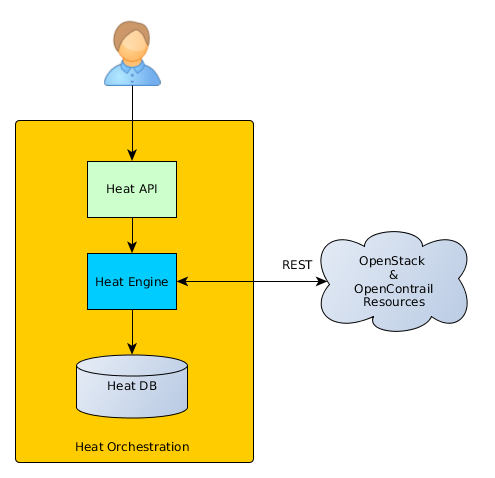
\includegraphics[scale=0.41]{images/heat_engine}
\par\end{centering}
\caption{Popis heat orchestrace\label{fig:heat_engine}}
\end{figure}

Z toho návrhu je patrné, že zde není implementovaný NFV orchestrator. Je to z důvodu toho, že pro účely řešení virtuálních síťových funkcí na cloudové platformě OpenStack s OpenContrailem, která je navržena v této práci, není tato část potřeba.

\subsection{Fyzicka topologie - underlay}\label{sub:interaction}

Celá testovací topologie se skládala z 4 serverů. Jeden server

\begin{figure}[h]
\begin{centering}
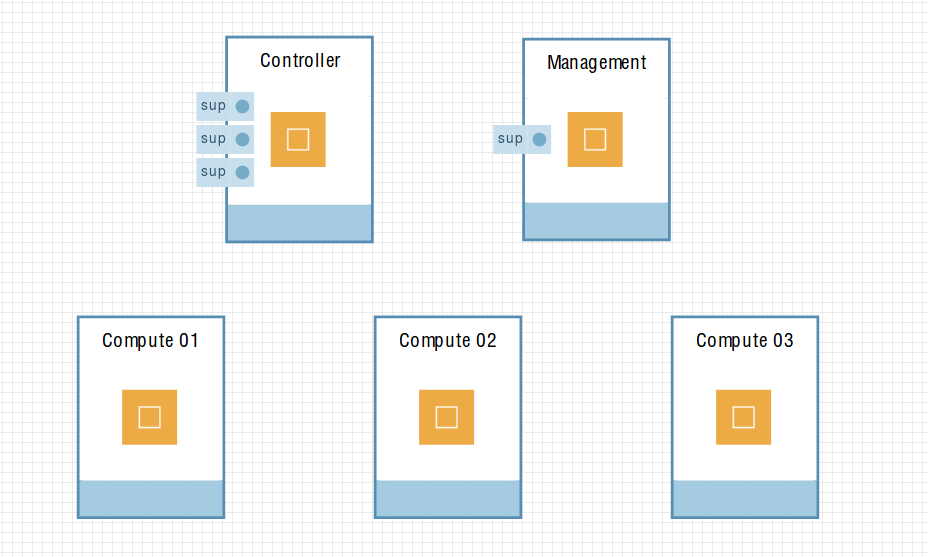
\includegraphics[scale=0.41]{images/ravello_topologie}
\par\end{centering}
\caption{Testovací topologie\label{fig:ravello_topologie}}
\end{figure}


\chapter{Testovací scénáře a realizace pro VNF a NFV}

V předchozí kapitole byla popsána oblast virtualizace síťových funkcí a jeji architektura. Také byly popsány jednotlivé technologie, které budou v této kapitole použity k realizaci ukázkových VNF. Pro každou VNF zde bude uveden příklad jejího použítí a jakým způsobem jsou realizovány požadavky na její životní cyclus, které byly uvedeny v předchozí kapitole.

\begin{figure}[h]
\begin{centering}
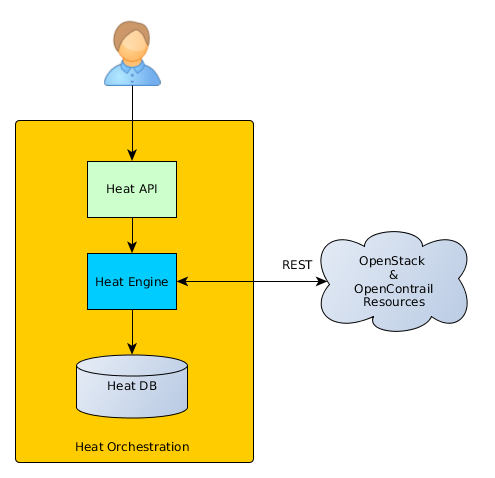
\includegraphics[scale=0.41]{images/heat_engine}
\par\end{centering}
\caption{Popis heat orchestrace\label{fig:heat_engine}}
\end{figure}

\section{Scenáře pro použití vybraných VNF}

\subsection{Scénář LbaaS}

Jedním z často využívaných síťových funkcí je load balancing. Pokud chce uživatel v cloudu provozovat nějaký druh webové služby, která musí být vysoce dostupná nebo bude velice vytížená, tak bude ve většině případů potřebovat využít více než jeden server. Pro rozdělení zátěže mezi tyto servery by následně použil fyzický load balancer. Ten bude spravovat příchozí komunikaci a distribuovat ji mezi několika serverů. Tím bude zajištěna rozloha zátěže a zajištěn bezvýpadkový provoz. Nevýhodou toho přístupu je právě nutnost pořízení fyzického load balanceru. Tím se uživatel značně omezí ve flexibilitě. Pokud například bude chtít další webové služby, které by měli být oddělené od těch stavajících, tak si bude muset opět pořizovat další hardwarový prvek. Alternativou k tomuto přístupu je využití cloudu a VNF, která bude mít load balancing funkcionalitu.

\begin{itemize}
\item Webové servery - Virtuální instance, na kterých bude umístěna požadovaná webová aplikace.
\item Privátní síť - Je síť, kde budou tyto servery umístěny.
\item Load balancer - Tato část je zodpovědná za řízení příchozí a odchozí komunikace webových serverů s okolním světem (Internetem).
\end{itemize}

\subsection{Scénář FwaaS}

\begin{figure}[h]
\begin{centering}
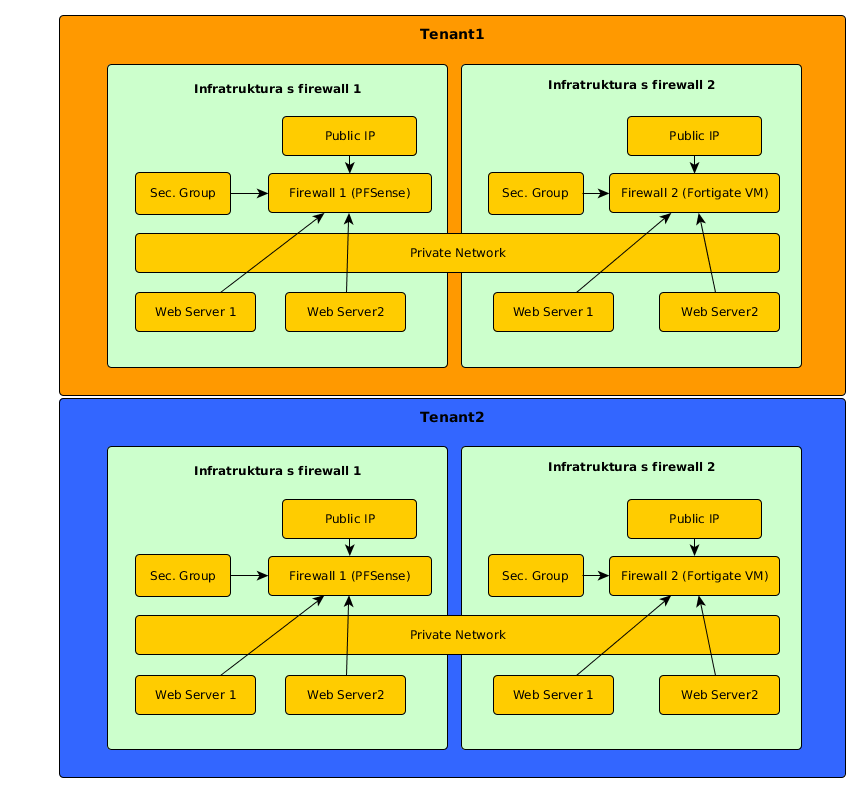
\includegraphics[scale=0.6]{images/firewall}
\par\end{centering}
\caption{Firewall as a Service\label{fig:firewall}}
\end{figure}

\section{Realizace VNF pro LbaaS}

\subsection{HAproxy - Neutron HAproxy agent}

OpenStack Neutron ve své implementaci obsahuje službu LBaaS. Je to jedna z jeho pokročilou služeb, která umožňuje použít jeden soubor API k ovládání load balanceru od poskytovatelů třetích stran. Jedinou podmínkou je, aby toto API implementovali. Toto velice zjednodušuje uživatelům OpenStacku ovládání load balancerů a odpadá díky tomu nutnost seznamování se s implementací a konfigurací těchto různých řešení, která mohou být velmi specifická a odlišná.

V této práci je ukázán příklad využítí implementace load balanceru v OpenContralu, který může být přes toto api ovládán. Tento příklad je však univerzální a může být použit s jakoukoli implementací load balanceru, at už virtuláního (sofwarového) či fyzického, pokud dokáže komunikovat s OpenStack Neutron LbaaS rozhraním. Dle dokumentace \cite{contrail_loadbalancer} je v OpenContrailu implementace load balanceru řešena pomocí HAProxy. HAProxy je zdarma dostupný open source software pro unix operační systémy \cite{HAProxy}. 

Load balancer se v Neutron LbaaS skládá ze 4 objektů.

\begin{itemize}
\item Pool - Označuje síťový rozsah pro webové servery.
\item Virtuální IP (VIP) - ip adresa, na kterou přichází komunikace
\item Member - Označuje konkrétní instanci, která je členem poolu.
\item Monitor - Monitoruje stav jednotlivých serverů a aplikací.
\end{itemize}

\begin{figure}[h]
\begin{centering}
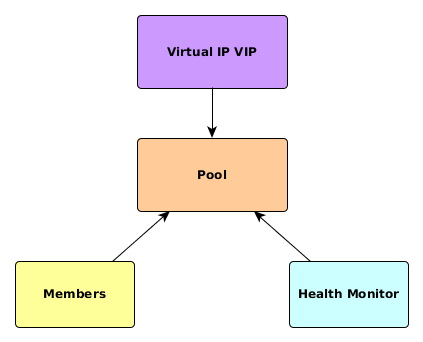
\includegraphics[scale=0.63]{images/NeutronLbaaS}
\par\end{centering}
\caption{Neutron LbaaS\label{fig:NeutronLbaaS}}
\end{figure}

Obrázek č. \ref{fig:NeutronLbaaS} zachycuje jednotlivé závislosti mezi těmito objekty. Tato implementace má tyto hlavní funkce:

\begin{itemize}
\item Poskytuje Load balancing komunikace od klientů do poolu serverů. Load balancer zprostředkovává spojení prostřednictvím své VIP.
\item Poskytuje load balancing pro HTTP, TCP a HTTPS komunikaci.
\item Poskytuje možnosti pro monitorování aplikací. Prostřednictvím HTTP, TCP či PING. Zde celý proces tak, že se load balancer pokusí v určeném časové intervalu navázat s daným serverem v pool spojení dle vybraného protokolu.
\item Umožňuje asociaci floating ip (veřejné adresy) k VIP, čímž umožňuje přístup k serverů z veřejné sítě.
\end{itemize}

Celý proces probíhá tak, že každý virtuální server, který je asociovaný s daným poolem z něj obdrží IP adresu. Když příjde na VIP nějaký dotaz na danou webovou aplikaci, tak je tento dotaz předán dál na jednu z těchto přiřazeným IP adres. Pokud nastane s aplikací či serverem nějaký problém, který zachytí monitor, tak load balancer ip adresu tohoto serveru přestane posílat komunikaci, dokud není vše zase v pořádku. Výběr serveru může probíhat pomocí jedné z následujících metod:

\begin{itemize}
\item Round robin - zde se komunikace distribuuje rovnoměrně, resp. dle vah zadaných u jednotlivých memberů v poolu.
\item Least connection - zde je vybran member s nejméně spojeními.
\item Source IP - u této metody je vybrán member na základě zdrojové ip adresy klienta.
\end{itemize}

V tomto případě si tedy není třeba starat o automatizaci konfigurace celého řešení. Je zde pouze nutné správně nadefinovat jednotlivé komponenty v heat templatu, abychom dosáhli požadovaného chování.

\subsubsection{LbaaS heat template}

Aby nemusel uživatel ručně vytvářet load balancer ručně, tak byl celý proces vytváření load balanceru zautomatizován pomocí heat templatu. Navržený heat template pro LbaaS v sobě obsahuje několik  prostředků, které se po jeho spuštění pokusí heat engine vytvořit. Celý template v sobě obsahuje i webové instance, které slouží pro testování. V produkci by však byly v odděleném templatu. Template je parametrizovaný a konktétní hodnoty pro jednotlivě zdroje (ip adresy, ip) jsou v tzv. enviroment file, který se zadává při spouštění daného templatu. Dále jsou popsány pouze hlavní části heat templatu.

\begin{itemize}
\item privatni síť - k této síti jsou připojeny obě webové instance, load balancer a router. Součástí je definice toho zdroje jsou je i subnet, který má dále paramentry týkající se DHCP ip adres.

\begin{lstlisting}[caption=Privátní síť a subnet]
private_net:
    type: OS::Neutron::Net
    properties:
      admin_state_up: True
      name: { get_param: private_net_name }
      shared: False
  private_subnet:
    type: OS::Neutron::Subnet
    properties:
      allocation_pools:
      - start: { get_param: private_net_pool_start }
        end: { get_param: private_net_pool_end }
      cidr: { get_param: private_net_cidr }
      enable_dhcp: True
      ip_version: 4
      name: { get_param: private_net_name }
      network_id: { get_resource: private_net }
\end{lstlisting}

\item 2 x web instance - jedná se o virtuální instance s operačním systémem Ubuntu 14.04. Po spuštění heat templatu se na tyto instance nainstaluje Apache server a vytvoří se index.html. Díky tomu je možné následně otestovat zda load balancer distubuje komunikaci mezi těmito dvěma servery.

\begin{lstlisting}[caption=Web server 1]
  instance_01:
    type: OS::Nova::Server
    properties:
      image: { get_param: instance_image }
      flavor: { get_param: instance_flavor }
      key_name: { get_param: key_name }
      name: test-web01
      networks:
      - network: { get_resource: private_net }
      security_groups:
      - default
      - { get_resource: http_security_group }
      user_data_format: RAW
      user_data: |
        #!/bin/bash -v
        apt-get install apache2 -yy
        echo "Instance 01" > /var/www/html/index.html
\end{lstlisting}


\item router - toto je Neutron router implementují SNAT. V tomto příkladě je využívaný webovými servery pro konektivitu k Internetu. Toto je nutné pro nainstalování programu Apache na webové servery.

\begin{lstlisting}[caption=Web server 1]
  router:
    type: OS::Neutron::Router
    properties:
      name: { get_param: router_name }
      external_gateway_info:
        network: { get_param: public_net_id }
\end{lstlisting}

\item public síť - toto je veřejná síť, ze které je získána VIP pro load balancer. Na tuto VIP bude dále asociována floating ip. 

\begin{lstlisting}[caption=Public síť a subnet]
  public_net:
    type: OS::Neutron::Net
    properties:
      admin_state_up: True
      name: { get_param: public_net_name }
      shared: False
  public_subnet:
    type: OS::Neutron::Subnet
    properties:
      allocation_pools:
      - start: { get_param: public_net_pool_start }
        end: { get_param: public_net_pool_end }
      cidr: { get_param: public_net_cidr }
      enable_dhcp: True
      ip_version: 4
      name: { get_param: public_net_name }
      network_id: { get_resource: public_net }
  lb_floating:
    type: OS::Neutron::FloatingIP
    properties:
      floating_network_id: {get_param: public_net_id}
      port_id: {get_attr: [lb_pool, vip, port_id]}
\end{lstlisting}

\item pool - jedná se o definování poolu pro load balancer. Na ukázce je vidět, že byla zvolena metoda Round Robin. Tato metoda byla zvolena kvůli co nejjednoduššímu testování tohoto templatu.

\begin{lstlisting}[caption=Load balancer pool]
  lb_pool:
    type: OS::Neutron::Pool
    properties:
      admin_state_up: True
      lb_method: ROUND_ROBIN
      name: { get_param: lb_name }
      protocol: HTTP
      monitors:
      - { get_resource: lb_ping_healt_monitor }
      subnet_id: { get_resource: private_subnet }
      vip:
        protocol_port: 80
        address: { get_param: public_net_ip }
        admin_state_up: True
        subnet: { get_resource: public_subnet }
\end{lstlisting}

\item members - po vytvoření instancí je nutné jejich přidání do poolu jako membery. Pokud webová aplikace na serverch využívá jiný port než port 80, je možné ho zde změnit.

\begin{lstlisting}[caption=Members]
  lb_pool_member_instance_01:
    type: OS::Neutron::PoolMember
    properties:
      address: { get_attr: [ instance_01 , first_address ] }
      admin_state_up: True
      pool_id: { get_resource: lb_pool }
      protocol_port: 80
\end{lstlisting}

\item health monitoring - zdroj pro monitoring. Dle zvolených parametrů je vidět, že každých 5 sekund bude poslán ping na servery a bude se čekat 5 sekund na odpověď. Pokud nepříjde, tak load balancer usoudí, že je daný server není v pořádku a přestane na něj přeposílat komunikaci.

\begin{lstlisting}[caption=Monitor]
  lb_ping_healt_monitor:
    type: OS::Neutron::HealthMonitor
    properties:
      admin_state_up: True
      delay: 5
      max_retries: 1
      timeout: 5
      type: PING
\end{lstlisting}
\end{itemize}

V celém heat templatu je ještě více zdrojů, které se vytváří. Ty zde však nebudou popsány. V případě zájmu lze nálest komletní heat template v příloze. 

\subsubsection{Testování LbaaS}\label{sub:interaction}

V reálné případě by si uživatel heat tempalte vybral z katalogu. Avšak v případě této práce bude heat template spouštěn pomocí příkazu v terminálu:

\begin{lstlisting}
heat stack-create -f heat/templates/lbaas_template.hot -e heat/env/lbaas_env.env lbaas
\end{lstlisting}

Tento příkaz vytvoří všechny již uvedené prostředky pro load balancing. Konkrétní load balancer má nakonfigurovanou virtual ip adresu (VIP) a k ní přiřazenou floating adresu, která je přístupná z externích sítí. Zároveň má tento load balancer přiřazený pool, ke kterému je přiřazena přiřazena privátní síť 10.10.10.0/24. Další zdrojem, který byl vytvořen je health monitor. Díky němu má load balancer přehled o aktuálním stavu webových instancí. Pokud by náhodou některá z nich přestala odpovídat, v tomto případě na ping, tak by load balancer na tuto instanci přestal zasílat traffic.

Na obrázku č. \ref{fig:lbaas_topologie} je zobrazek screenshot vytvořené topologie v OpenStack dashboardu. Jsou zde vidět vytvořené servery a sítě. Není zde zobrazen load balancer, protože tato vizualizace tento prvek nezobrazuje. Lze ho nalézt v jiné části dashboardu, ale pro názornost bude rovnou otestováno jeho správné chování.

\begin{figure}[h]
\begin{centering}
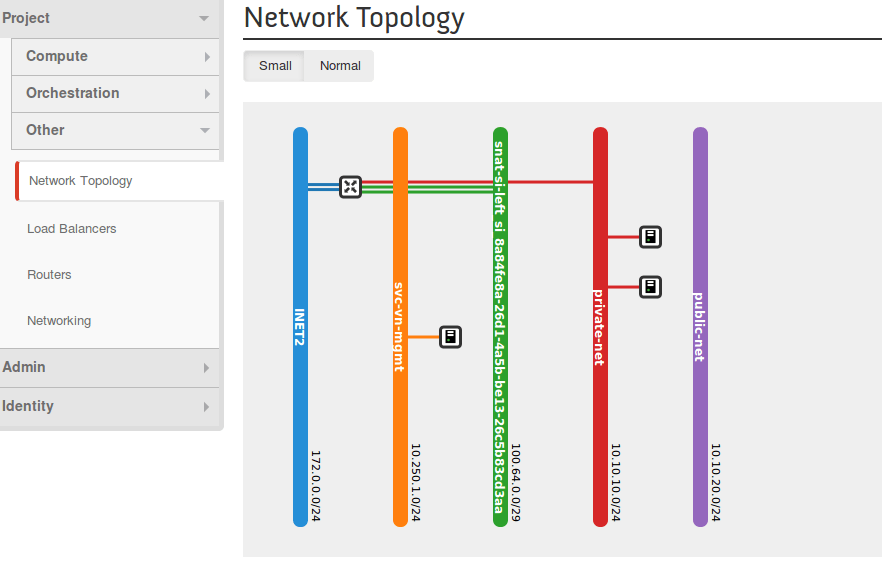
\includegraphics[scale=0.45]{images/lbaas_topologie}
\par\end{centering}
\caption{Vytvořená síťová topologie\label{fig:lbaas_topologie}}
\end{figure}

Otestování správného chování virtuálního load balanceru, lze provést opakovaným dotazem na právě vytvořené webové servery. Tím je bude zároveň otestována jejich správná konfigurace. Pokud by totiž nevrátili správnou odpoveď je možné, že chyba může být i zde. 

Dotaz na webové servery byl proveden pomocí příkazu curl, kterému byla dána jako parametr public adresa load balanceru. Celý výstup toho testování znázorňuje obrázek č. \ref{fig:lbaas_testing}. Po několika takovýchto dotazech na webové servery je vidět, že odpověď příchází střídavě od obou webových serverů. Probíhá mezi nimi tedy load balancing metodou round robin tak, jak bylo požadováno.

\begin{figure}[h]
\begin{centering}
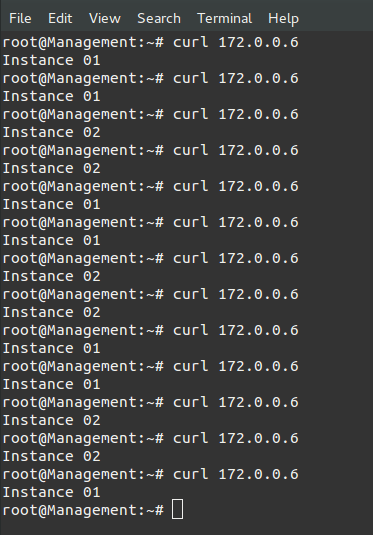
\includegraphics[scale=0.3]{images/lbaas_testing}
\par\end{centering}
\caption{Test konektivity a load balancingu\label{fig:lbaas_testing}}
\end{figure}


\subsection{AVI networks}

\section{Realizace VNF pro FwaaS}

\subsection{Heat template}

Pro FwaaS je narhnut heat template, který obsahuje:

\begin{itemize}

\item privátní síť


\begin{lstlisting}[caption=Privátní síť]
  private_net_1:
    type: OS::Neutron::Net
    properties:
      name: { get_param: private_net_1_name } 

  private_subnet_1:
    type: OS::Neutron::Subnet
    depends_on: private_net_1
    properties:
      network_id: { get_resource: private_net_1 }
      cidr: { get_param: private_net_1_cidr }
      gateway_ip: { get_param: private_net_1_gateway }
      allocation_pools:
        - start: { get_param: private_net_1_pool_start }
          end: { get_param: private_net_1_pool_end }
\end{lstlisting}


\item firewall template

\begin{lstlisting}[caption=Firewall servisní instance]
service_template:
    type: OS::Contrail::ServiceTemplate
    properties:
      name: { get_param: template_name }
      service_mode: { get_param: template_mode }
      service_type: { get_param: template_type }
      image_name: { get_param: template_image }
      service_scaling: { get_param: scaling }
      availability_zone_enable: { get_param: availability_zone }
      ordered_interfaces: { get_param: ordered_interfaces }
      flavor: { get_param: template_flavor }
      service_interface_type_list: { "Fn::Split" : [ ",", Ref: service_interface_type_list ] }
      shared_ip_list: { "Fn::Split" : [ ",", Ref: shared_ip_list ] }
      static_routes_list: { "Fn::Split" : [ ",", Ref: static_routes_list ] }

\end{lstlisting}

\item firewall instance
\begin{lstlisting}[caption=Privátní síť]
 service_instance:
    type: OS::Contrail::ServiceInstance
    depends_on: [private_subnet_1]
    properties:
      name: { get_param: private_instance_name }
      service_template: { get_resource:  service_template}
      availability_zone: { get_param: private_availability_zone}
      scale_out: 
          max_instances: { get_param: max_instances }
      interface_list: [
          {
              virtual_network: "auto"
          },
          {
              virtual_network: {get_param: public_net}
          },
          {
              virtual_network: {get_resource: private_net_1}
          }
      ]
\end{lstlisting}


\item virtuální instance
\begin{lstlisting}[caption=Virtuální instance pro testování]

 test_instance_01:
    type: OS::Nova::Server
    properties:
      image: { get_param: instance_image }
      flavor: { get_param: instance_flavor }
      key_name: { get_param: key_name }
      name: test-web01
      networks:
      - network: { get_resource: private_net_1 }
      security_groups:
      - default
      user_data_format: RAW
      user_data: |
        #!/bin/bash -v
        apt-get install apache2 -yy
        echo "Instance 01" > /var/www/html/index.html

\end{lstlisting}

\item contrail policy

\begin{lstlisting}[caption=Contrail network policy]

  private_policy:
    type: OS::Contrail::NetworkPolicy
    depends_on: [ private_net_1, service_instance ]
    properties:
      name: { get_param: policy_name }
      entries:
        policy_rule: [
              { 
                "direction": { get_param: direction }, 
                "protocol": "any", 
                "src_ports": [{"start_port": {get_param: start_src_ports}, "end_port": {get_param: end_src_ports}}],
                "dst_ports": [{"start_port": {get_param: start_dst_ports}, "end_port": {get_param: end_dst_ports}}],
                "dst_addresses": [{ "virtual_network": {get_param: public_net}}], 
                "action_list": {"apply_service": [{get_resource: service_instance}]}, 
                "src_addresses": [{ "virtual_network": {get_resource: private_net_1}}] 
              }, 
        ]

\end{lstlisting}
\end{itemize}

\subsection{PfSense}

//Bash script nefunguje
//Predpripraveny image

\subsection{Fortigate}

//Python API = Script
// => Salt module 

\section{Tvorba Firewall as a Service}

Další velmi častou síťovou funkcí, která je často využívána je firewall. 

V tomto případě má tedy každý uživatel cloudu možnost si vytvořit vlastní servisní instanci.  

Největší výhodou použití firewall VNF v OpenContrailu je možnost nasazení tohoto firewallu ve vysoké dostupnosti.

Dalším častým příklad VNF, kterou uživatelé cloudu mohou potřebovat je firewall. Oproti LbaaS je zde situace o něco komplikovanější. Je zde totiž více možností a jak daný firewall využívat. U tohoto příkladu služby bude uvedeno několik scénářů, které 

\subsection{Servisní instance v OpenContrailu}

V OpenContrailu je sice možnost využívat implementaci routeru s SNAT, která umožnuje instancím v privátních sítích konektivitu s externí sítí. Pokud však uživatel potřebuje využít pokročilejší funkce firewallu, tak je možné vytvořit servisní instanci, která bude sloužit jako VNF. V té může být použit libovolný požadovaný image firewallu uživatele.

Servisní instance v OpenContrailu je jednoduše virtuální stroj, který poskytuje danou VNF. Úplně nejjednodušším příkladem může být virtuální stroj s operačním systémem GNU/Linux, který může sloužit jako router mezi dvěma sítěmi. Pro vytvoření takového virtuálního stroje jsou nutné 3 základní elementy. 

\begin{itemize}
 	\item Service Template
  \item Service Instance
  \item Service Policy
\end{itemize}

Servisní Template obsahuje obecný předpis pro danou VNF v OpenContrailu. Pro správné fungování je nutné zadat nastavit správné parametry patří:

\begin{itemize}
\item Název - Název je označení daného Servisního Templatu. Pomocí něho lze následně identifikovat daný template a spustit dle jeho parametrů Servisní instanci. 
\item Image - Je image, který má být použit pro vytvoření dané servisní instance. V našem případě se bude jednat o image, který obsahuje požadované síťové funkce. Tento image musí před tím než může být použit  nahrán do OpenStacku Glance.
\item Service Type - V OpenContrailu, prozatím existují dva typy. Jsou to Trafic Analyzer a Firewall.
\item Service Mode - Zde se určuje v jakém modu daný template bude nastaven. Jsou zde 3 možnosti. , .

	\begin{itemize}
	\item Transparent - v tomto případě se jedná o neroutovaný firewall, neboli L2 firewall.
	\item In-Network - poskytuje výchozí bránu a průchozí traffic je routovaný. Tento mode může být využit pro NAT, HTTP proxy, atd.
	\item In-Network-NAT - zde je situace podobná jako u In-Network, ale navracející traffic nemusí být routovaný zpět do zdrojové sítě.
	\end{itemize}

\item Typy síťových portů - Zde se určuje kolik portů bude daná instance, vytvořená pomocí tohoto templatu mít a jaká bude jejich role. Jsou zde možnosti Left, Right a Management. 
\end{itemize}

Po úspěšném vytvoření Servisního templatu je možné z něj vytvořit libovolný počet Servis Instancí.  Ty běží jako klasické instance v OpenStacku. Jak tedy vyplývá z výše uvedených informací, tak existují dva druhy servisních instancí v OpenContrailu. 

První z nich je Analyzer. Ten slouží k analýze a zachytávání síťového trafficu. Image pro tento typ servisní instance obvykle obsahuje protokolový analyzér a paketový sniffer, jako je například oblíbený program Wireshark. Tato instance dostává traffic, který je posílán mezi dvěma sítěmi. Tento traffic vybírá OpenContrail podle nastaveného pravidla pro dané sítě. Podle těchto pravidel je vybrána jen část trafficu, která je následně dána k dispozici servisní instanci. Samotná servisní instance nijak nemanipuluje s trafficem a ani do něj žádný negeneruje. Jednoduše lze říci, že má nastavený síťový port v promiskuitním modu a pouze pozoruje traffic. Poté jen hlásí zachycené události uživateli čí jiným entitám v síti. Obrázek č. \ref{fig:service_instance_anal} znázorňuje tento typ servisní instance.

\begin{figure}[h]
\begin{centering}
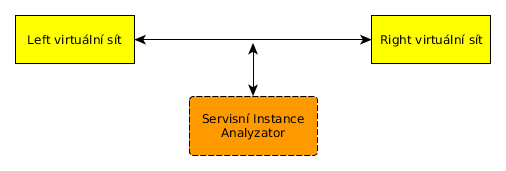
\includegraphics[scale=0.63]{images/service_instance_anal}
\par\end{centering}
\caption{Schéma zapojení servisní instance Analyzer\label{fig:service_instance_anal}}
\end{figure}

Druhým typen servisní instance je firewall. V tomto případě již servisní instance manipuluje s trafficem. Hlavní bodem při vytváření servisní instance jako firewall je přiřadit správné virtuální sítě k správným virtuálním síťovým portům. Servisní instance má obvykle dva síťové porty - left a right. Ty slouží pro propojení sítí do kterých jsou zapojeny. V některých případech je možné servisní instanci přidat třetí síťový port, který slouží pro out-of-band management. Přestože některá řešení pro servisní instance sloužící jako firewall mohou mít již své požadované chování definované hned při jejich startu, tak tento port může být velice užitečný při konfiguraci dané servisní instance. A to ať už se jedná o konfiguraci manuální či pomocí nějaké vyšší management entity.

\begin{figure}[h]
\begin{centering}
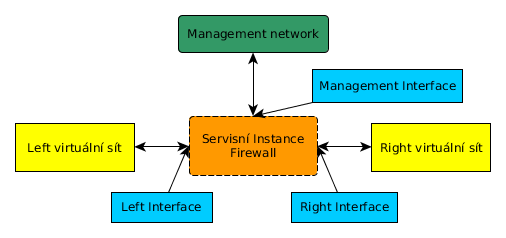
\includegraphics[scale=0.63]{images/service_instance}
\par\end{centering}
\caption{Schéma zapojení servisní instance\label{fig:service_instance}}
\end{figure}


Service policy dovoluje síťový traffic mezi virtuálními sítěmi a říká systému, aby ho posílal skrze servisní instanci.



\subsection{Testování FwaaS s PfSense}\label{sub:interaction}

Pro vytvoření heat stacku s PFSense z templatu lze použít příkaz:

\verb!heat stack-create -f heat/templates/fwaas_mnmg_template.hot -e heat/env/fwaas_pfsense_env.env pfsense!

a pro vytvoření heat stacku s Fortigate VM jde vytvořit pomocí příkazu:

\verb!heat stack-create -f heat/templates/fwaas_mnmg_template.hot -e heat/env/fwaas_fortios_contrail.env fortios!


\begin{figure}[h]
\begin{centering}
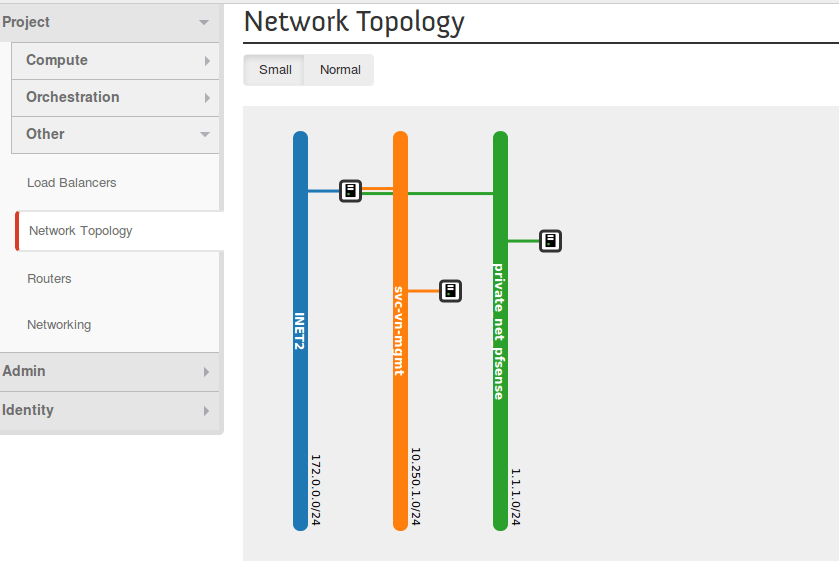
\includegraphics[scale=0.45]{images/fwaas_topologie}
\par\end{centering}
\caption{Síťová topologie\label{fig:fwaas_topologie}}
\end{figure}


By default, pfsense firewall is configured to NAT after the heat stack is started. As a result, there is no need to make any configuration for this function. Pfsense image was preconfigured with DHCP services on every interface and there is outbound policy for NAT.

After we start the heat with pfsense there is already functional service chaining. Testing instance has default gateway to contrail and contrail redirects it to pfsense.

\begin{figure}[h]
\begin{centering}
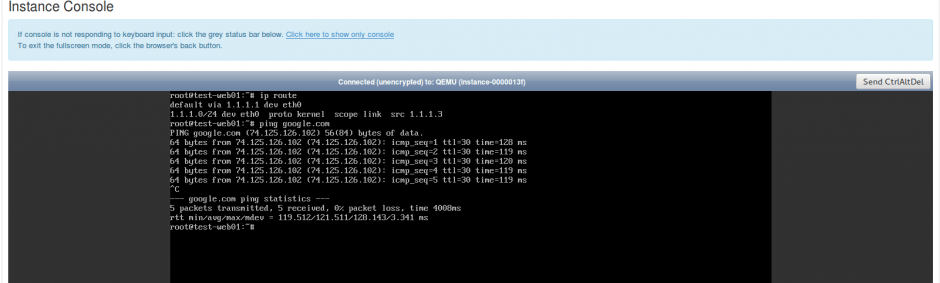
\includegraphics[scale=0.45]{images/pfsense_ping}
\par\end{centering}
\caption{Test konektivity PFSense\label{fig:pfsense_ping}}
\end{figure}

\begin{figure}[h]
\begin{centering}
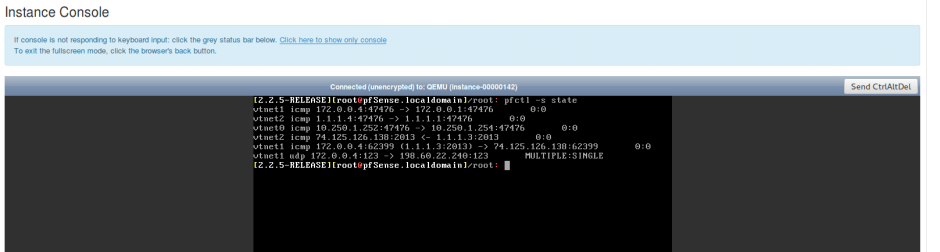
\includegraphics[scale=0.45]{images/pfsense_nat}
\par\end{centering}
\caption{Ukázka NAT session\label{fig:pfsense_nat}}
\end{figure}


\subsection{Testování FwaaS s Fortigate}\label{sub:interaction}

\begin{figure}[h]
\begin{centering}
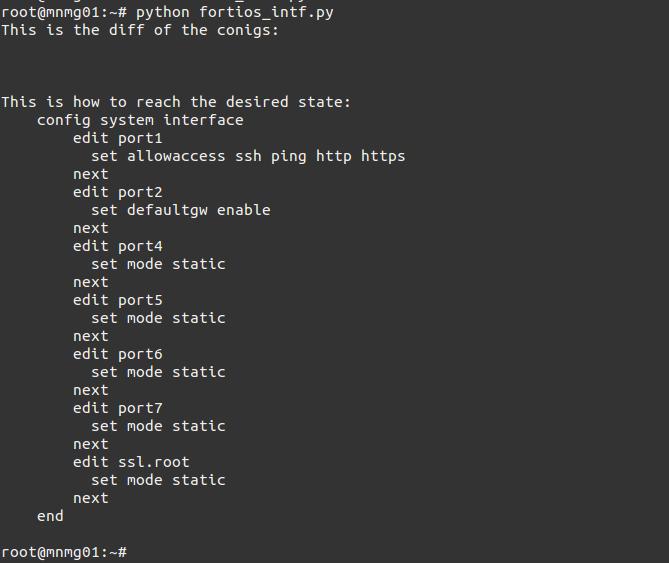
\includegraphics[scale=0.45]{images/fortigate_int}
\par\end{centering}
\caption{Fortigate VM intergace konfigurace\label{fig:fortigate_int}}
\end{figure}

\begin{figure}[h]
\begin{centering}
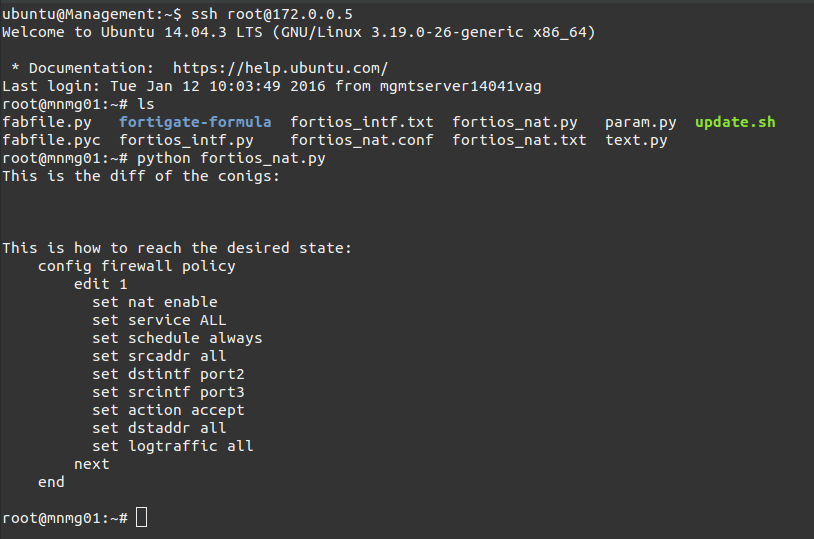
\includegraphics[scale=0.45]{images/fortigate_nat}
\par\end{centering}
\caption{Fortigate VM NAT konfigurace\label{fig:fortigate_nat}}
\end{figure}

\begin{figure}[h]
\begin{centering}
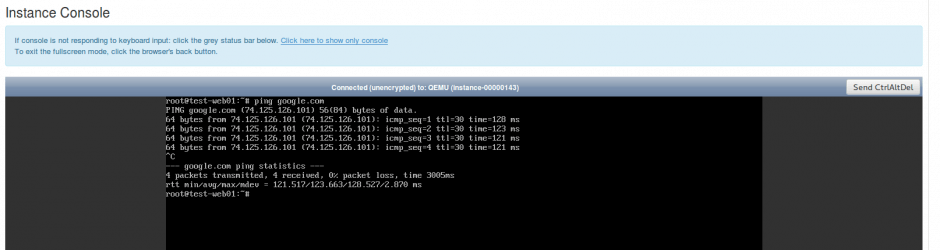
\includegraphics[scale=0.45]{images/fortigate_ping}
\par\end{centering}
\caption{Test konektivity\label{fig:fortigate_ping}}
\end{figure}


\chapter{Závěr}

Je v paráda.


\cleardoublepage{}
\appendix
\pagenumbering{Roman}

%<------------------------------bibliography------------------------------------>

\addcontentsline{toc}{part}{Literatura} \renewcommand{\appendixname}{Literatura}%%přílohy, číslování římskými

%<------------------------------bibliography------------------------------------>
\bibliographystyle{ieeetr}  
\begin{thebibliography}{10}

\bibitem{Cloud_adoption}\url{http://www.rightscale.com/blog/cloud-industry-insights/cloud-computing-trends-2016-state-cloud-survey}

\bibitem{SDN_adoption}\url{}

\bibitem{NFV_challages}

\bibitem{NFV_paper2012}R. Guerzoni, “Network Functions Virtualisation: An Introduction, Benefits, Enablers, Challenges and Call for Action. Introductory white paper,” in SDN and OpenFlow World Congress, June 2012. [online]. [cit. 2016-04-07]. Dostupné také z: \url{https://portal.etsi.org/NFV/NFV_White_Paper.pdf}

\bibitem{NFV_paper2013}

\bibitem{}

\bibitem{OPNFV}Open plateform for nfv. \url{https://www.opnfv.org/}.  Accessed September 28,
2014.

\bibitem{NFVState}MIJUMBI, Rashid, Joan SERRAT, Juan-Luis GORRICHO, Niels BOUTEN, Filip DE TURCK a Raouf BOUTABA. \emph{Network Function Virtualization: State-of-the-Art and Research Challenges.} IEEE Communications Surveys. 2016, 18(1), 236-262. DOI: 10.1109/COMST.2015.2477041. ISSN 1553-877x. Dostupné také z: \url{http://ieeexplore.ieee.org/lpdocs/epic03/wrapper.htm?arnumber=7243304}

\bibitem{NFVChalanges}HAN, Bo, Vijay GOPALAKRISHNAN, Lusheng JI a Seungjoon LEE. \emph{Network function virtualization: Challenges and opportunities for innovations}. IEEE Communications Magazine. 2015, 53(2), 90-97. DOI: 10.1109/MCOM.2015.7045396. ISSN 0163-6804. Dostupné také z: \url{http://ieeexplore.ieee.org/lpdocs/epic03/wrapper.htm?arnumber=7045396}

\bibitem{VM_book}KUSNETZKY, Dan. \emph{Virtualization: a manager's guide}. Sebastopol, CA: O'Reilly, c2011. ISBN 1449306454.

\bibitem{VM_architektura}J. Smith and R. Nair, “The architecture of virtual machines,” Computer, vol. 38, no. 5, pp. 32–38, May 2005. doi: 10.1109/MC.2005.173

\bibitem{Cloud_book}K. Chandrasekaran. \emph{Essentials of CLOUD COMPUTING}. Boca Raton: CRC Press, 2015. ISBN 978-1-4822-0544-2.

\bibitem{CloudSurvey}JENNINGS, Brendan a Rolf STADLER. \emph{Resource Management in Clouds: Survey and Research Challenges}. Journal of Network and Systems Management. 2015, 23(3), 567-619. DOI: 10.1007/s10922-014-9307-7. ISSN 1064-7570. Dostupné také z: \url{http://link.springer.com/10.1007/s10922-014-9307-7}

\bibitem{NFV_use_cases}ETSI, “Network Function Virtualization: Use Cases”, \url{http://www.etsi.org/deliver/etsi_gs/NFV/001_099/001/01.01.01_60/gs_NFV001v010101p.pdf}, 2013

\bibitem{SDN_clanek}KREUTZ, Diego, Fernando M. V. RAMOS, Paulo ESTEVES VERISSIMO, Christian ESTEVE ROTHENBERG, Siamak AZODOLMOLKY a Steve UHLIG. \emph{Software-Defined Networking: A Comprehensive Survey}. Proceedings of the IEEE [online]. 2015, 103(1), 14-76 [cit. 2016-04-09]. DOI: 10.1109/JPROC.2014.2371999. ISSN 0018-9219. Dostupné z: \url{http://ieeexplore.ieee.org/lpdocs/epic03/wrapper.htm?arnumber=6994333}

\bibitem{SDN_book} DOHERTY, Jimmy. \emph{SDN and NFV simplified: a visual guide to understanding software defined networks and network function virtualization}. 1st edition. Indianapolis, IN: Addison-Wesley Professional, 2016. ISBN 9780134306407.

\bibitem{NFV_architektura}ETSI Industry Specification Group (ISG) NFV, “ETSI GS NFV 002 V1.2.1: Network Functions Virtualisation (NFV); Architectural Framework,” December 2014. [online]. [cit. 2016-04-07]. Dostupné také z: \url{http://www.etsi.org/deliver/etsi gs/NFV/001 099/002/01. 02.01 60/gs NFV002v010201p.pdf} 

\bibitem{NFV_terminology}ETSI Industry Specification Group (ISG) NFV, “ETSI GS NFV 003 V1.2.1: Network Functions Virtualisation (NFV); Terminology for Main Concepts in NFV,” December 2014. [online]. [cit. 2016-04-07]. \url{ttp://www.etsi.org/deliver/etsi gs/NFV/001099/003/01.02.01 60/gs NFV003v010201p.pdf}

\bibitem{NFV_infrastructure}\url{http://www.etsi.org/deliver/etsi_gs/NFV-INF/001_099/001/01.01.01_60/gs_nfv-inf001v010101p.pdf}

\bibitem{NFV_compute} \url{http://www.etsi.org/deliver/etsi_gs/NFV-INF/001_099/003/01.01.01_60/gs_NFV-INF003v010101p.pdf}

\bibitem{NFV_hypervisor} \url{http://www.etsi.org/deliver/etsi_gs/NFV-INF/001_099/004/01.01.01_60/gs_nfv-inf004v010101p.pdf}

\bibitem{NFV_network} \url{http://www.etsi.org/deliver/etsi_gs/NFV-INF/001_099/005/01.01.01_60/gs_NFV-INF005v010101p.pdf}

\bibitem{NFV_VNF}\url{http://www.etsi.org/deliver/etsi_gs/NFV-SWA/001_099/001/01.01.01_60/gs_nfv-swa001v010101p.pdf}

\bibitem{NFV_MANO}\url{http://www.etsi.org/deliver/etsi_gs/NFV-MAN/001_099/001/01.01.01_60/gs_nfv-man001v010101p.pdf}

\bibitem{NFV_orchestration}MIJUMBI, Rashid, Joan SERRAT, Juan-luis GORRICHO, Steven LATRE, Marinos CHARALAMBIDES a Diego LOPEZ. \emph{Management and orchestration challenges in network functions virtualization}. IEEE Communications Magazine. 2016, 54(1), 98-105. DOI: 10.1109/MCOM.2016.7378433. ISSN 0163-6804. Dostupné také z: \url{http://ieeexplore.ieee.org/lpdocs/epic03/wrapper.htm?arnumber=7378433}

\bibitem{OpenStack} KHEDHER, Omar. \emph{Mastering OpenStack: design, deploy, and manage a scalable OpenStack infrastructure}. First published. Birmingham: Packt Publishing, 2015. Community experience distilled (Packt). ISBN 978-1-78439-564-3.

\bibitem{OpenStack2}JACKSON, Kevin. \emph{OpenStack cloud computing cookbook}. Third Edition. Birmingham: Packt Publishing, 2015. ISBN 978-1-78217-478-3.

\bibitem{OpenContrail} RIJSMAN, Bruno a Ankur SINGLA. \emph{Day One: Understanding OpenContrail Architecture}. Juniper Networks Books, 2013

\bibitem{OpenContrail2} Architecture   Dokumentation.   SINGLA,   Ankur   a   Bruno   RIJSMAN. \emph{OpenContrail}. [online].  Juniper  Networks  Books,   2013  [cit.2016-04-04]. Dostupné    z: \url{http://www.opencontrail.org/opencontrail-architecture-documentation/}

\bibitem{contrail_loadbalancer}

\bibitem{pfsense}

\bibitem{fortigate}

\bibitem{heat}

\bibitem{contrail_service}

\bibitem{contrail_ha_firewall}

\bibitem{HAProxy}

\end{thebibliography}

\cleardoublepage{}

\listoffigures

%\addcontentsline{toc}{part}{Seznam obrázků}{12} \renewcommand{\appendixname}{Seznam obrázků}%

\listoftables

%\addcontentsline{toc}{part}{Seznam tabulek} \renewcommand{\appendixname}{Seznam tabulek}%

\lstlistoflistings

%\addcontentsline{toc}{part}{Seznam ukázek kódu} \renewcommand{\appendixname}{Seznam ukázek kódu}%

\addcontentsline{toc}{part}{Přílohy}\thispagestyle{empty}  \renewcommand{\appendixname}{P\v{r}iloha}%%přílohy, číslování římskými
\part*{Přílohy} %% rename
\appendix
\chapter{Heat template Lbaas - HAproxy}

\begin{lstlisting}
heat_template_version: 2013-05-23
description: LBAAS Template
parameters:
  key_name:
    type: string
  instance_flavor:
    type: string
    description: Instance type for servers
    default: m1.small
    constraints:
      - allowed_values: [m1.tiny, m1.small, m1.medium, m1.large]
        description: instance_type must be a valid instance type
  instance_image:
    type: string
    description: Image name to use for the servers.
    default: ubuntu-14-04-x64
  public_net_id:
    type: string
    description: ID or name of public network for which floating IP addresses will be allocated
  router_name:
    type: string
    description: Name of router to be created
    default: test-router
  lb_name:
    type: string
    description: Name of balancer to be created
    default: test-lb
  public_net_name:
    type: string
    description: Name of public network to be created
    default: public-net
  public_net_cidr:
    type: string
    description: Public network address (CIDR notation)
    default: 10.10.20.0/24
  public_net_pool_start:
    type: string
    description: Start of public network IP address allocation pool
    default: 10.10.20.100
  public_net_pool_end:
    type: string
    description: End of public network IP address allocation pool
    default: 10.10.20.200
  private_net_name:
    type: string
    description: Name of private network to be created
    default: private-net
  private_net_cidr:
    type: string
    description: Private network address (CIDR notation)
    default: 10.10.10.0/24
  private_net_pool_start:
    type: string
    description: Start of private network IP address allocation pool
    default: 10.10.10.100
  private_net_pool_end:
    type: string
    description: End of private network IP address allocation pool
    default: 10.10.10.200
resources:
  http_security_group:
    type: OS::Neutron::SecurityGroup
    properties:
      name: http
      rules:
      - direction: ingress
        remote_mode: remote_ip_prefix
        remote_ip_prefix: 0.0.0.0/0
        port_range_min: 80
        port_range_max: 80
        protocol: tcp
  public_net:
    type: OS::Neutron::Net
    properties:
      admin_state_up: True
      name: { get_param: public_net_name }
      shared: False
  public_subnet:
    type: OS::Neutron::Subnet
    properties:
      allocation_pools:
      - start: { get_param: public_net_pool_start }
        end: { get_param: public_net_pool_end }
      cidr: { get_param: public_net_cidr }
      enable_dhcp: True
      ip_version: 4
      name: { get_param: public_net_name }
      network_id: { get_resource: public_net }
  private_net:
    type: OS::Neutron::Net
    properties:
      admin_state_up: True
      name: { get_param: private_net_name }
      shared: False
  private_subnet:
    type: OS::Neutron::Subnet
    properties:
      allocation_pools:
      - start: { get_param: private_net_pool_start }
        end: { get_param: private_net_pool_end }
      cidr: { get_param: private_net_cidr }
      enable_dhcp: True
      ip_version: 4
      name: { get_param: private_net_name }
      network_id: { get_resource: private_net }
  router:
    type: OS::Neutron::Router
    properties:
      name: { get_param: router_name }
      external_gateway_info:
        network: { get_param: public_net_id }
  router_interface:
    type: OS::Neutron::RouterInterface
    properties:
      router_id: { get_resource: router }
      subnet_id: { get_resource: private_subnet }
  lb_ping_healt_monitor:
    type: OS::Neutron::HealthMonitor
    properties:
      admin_state_up: True
      delay: 5
      max_retries: 1
      timeout: 5
      type: PING
  lb_pool:
    type: OS::Neutron::Pool
    properties:
      admin_state_up: True
      lb_method: ROUND_ROBIN
      name: { get_param: lb_name }
      protocol: HTTP
      monitors:
      - { get_resource: lb_ping_healt_monitor }
      subnet_id: { get_resource: private_subnet }
      vip:
        protocol_port: 80
#        address: { get_param: public_net_ip }
        admin_state_up: True
        subnet: { get_resource: public_subnet }
  instance_01:
    type: OS::Nova::Server
    properties:
      image: { get_param: instance_image }
      flavor: { get_param: instance_flavor }
      key_name: { get_param: key_name }
      name: test-web01
      networks:
      - network: { get_resource: private_net }
      security_groups:
      - default
      - { get_resource: http_security_group }
      user_data_format: RAW
      user_data: |
        #!/bin/bash -v
        apt-get install apache2 -yy
        echo "Instance 01" > /var/www/html/index.html
  lb_pool_member_instance_01:
    type: OS::Neutron::PoolMember
    properties:
      address: { get_attr: [ instance_01 , first_address ] }
      admin_state_up: True
      pool_id: { get_resource: lb_pool }
      protocol_port: 80
      weight: 1
  instance_02:
    type: OS::Nova::Server
    properties:
      image: { get_param: instance_image }
      flavor: { get_param: instance_flavor }
      key_name: { get_param: key_name }
      name: test-web02
      networks:
      - network: { get_resource: private_net }
      security_groups:
      - default
      - { get_resource: http_security_group }
      user_data_format: RAW
      user_data: |
        #!/bin/bash -v
        apt-get install apache2 -yy
        echo "Instance 02" > /var/www/html/index.html
  lb_pool_member_instance_02:
    type: OS::Neutron::PoolMember
    properties:
      address: { get_attr: [ instance_02 , first_address ] }
      admin_state_up: True
      pool_id: { get_resource: lb_pool }
      protocol_port: 80
      weight: 1
  lb:
    type: OS::Neutron::LoadBalancer
    properties:
      members:
      - { get_resource: instance_01 }
      - { get_resource: instance_02 }
      pool_id: { get_resource: lb_pool }
      protocol_port: 80
  lb_floating:
    type: OS::Neutron::FloatingIP
    properties:
      floating_network_id: {get_param: public_net_id}
      port_id: {get_attr: [lb_pool, vip, port_id]}
\end{lstlisting}

\chapter{Heat template FwaaS}



%<------------------------------external PDF------------------------------------>
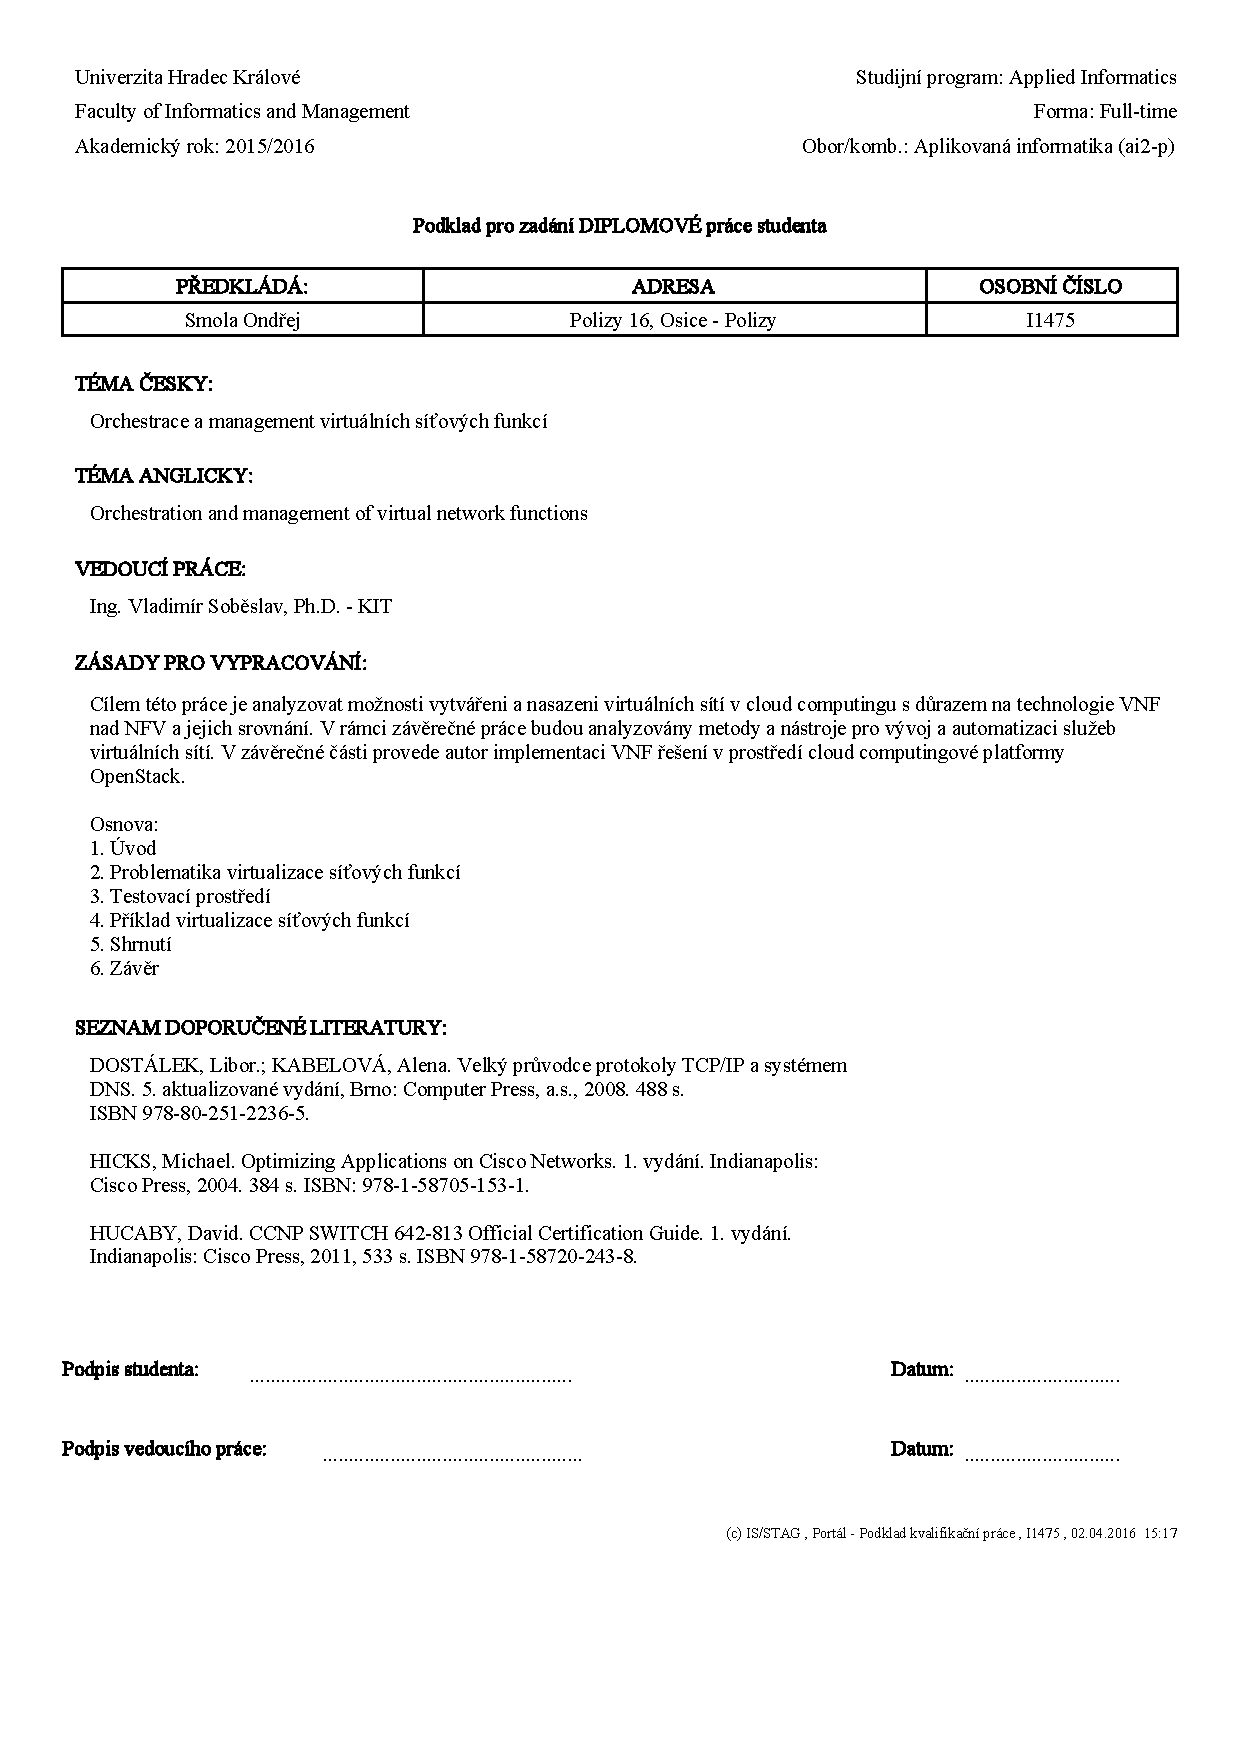
\includepdf[pages={1}]{zadani.pdf}

\end{document}
